
\chapter{Implementing VEP-based brain-computer interface}

The previous chapter discussed the biology of the brain and described the brain potential called \gls{SSVEP}. The aim of this chapter is to describe which kind of visual stimuli can be used to elicit an \gls{SSVEP} and how to detect the elicited \gls{SSVEP} in the \gls{EEG} recording. This knowledge is needed to extract information from the \gls{EEG} recording and use this information to control a robot. In other words, this chapter will discuss how to implement a \gls{VEP}-based \gls{BCI}.

\section{Designing visual stimuli}
\label{sec:stimuli}

As discussed in section~\ref{sec:VEP}, it is possible to present multiple visual stimuli to a subject and detect, which stimulus is the subject looking at. It was also mentioned that computer monitor can be used to present visual stimuli. This section will discuss how stimuli with certain blinking frequency can be displayed by a computer monitor.

Research has shown that LCD screens produce more reliable \gls{SSVEP} response than \gls{LED}~\cite{lcd_lcd_led}. Another article, however, concludes that \glspl{BCI} that use \glspl{LED} as visual stimuli have achieved better performance~\cite{ssvep_stim}. But since using \glspl{LED} requires dedicated hardware, only the stimuli that can be displayed by a computer monitor are discussed in this thesis.

A computer monitor has certain size, resolution and \gls{refresh rate}. Monitor resolution and size limit the size of the visual stimuli that can be used and the distance between the stimuli. Monitor \gls{refresh rate}, on the other hand, limits the presentation rate or blinking frequency of the stimulus that can be used. Research has shown that LCD screens produce more reliable \gls{SSVEP} response when using monitor \gls{refresh rate} for measuring the time between stimuli presentations rather than a timer~\cite{lcd_lcd_led}. Therefore, monitor \gls{refresh rate} is used for timing and synchronisation also in this thesis.

Monitor \gls{refresh rate} is the number of consecutive images or \glspl{frame} shown on the screen in a second, assuming that the \glspl{frame} are produces at least as fast as they can be displayed. A \gls{frame} is one of the images that compose the changing picture on the screen. Monitor with a \gls{refresh rate} of \SI{60}{Hz} can display 60 \glspl{frame} per second. 

Often blinking one-coloured squares on one-coloured background are used as visual stimuli in \gls{SSVEP}-based \glspl{BCI}~\cite{ssvep_stim}. The squares may have symbols on them, for example letters or numbers. The stimuli of \gls{VEP}-based \gls{BCI} are also called \glspl{target} and the blinking of a \gls{target} is called \gls{flickering}.

In every \gls{frame} each \gls{target} can be in one of two \glspl{state}---displayed or not displayed. The \gls{state} of a \gls{target} can be switched only when the current \gls{frame} is replaced with the next \gls{frame}. The \gls{state} switches should be distributed as evenly as possible for the \gls{target} frequency to be constant. Distributing the \gls{state} switches is easier with some frequencies than others. For example, if \gls{refresh rate} is \SI{60}{Hz}, then
\begin{itemize}
	\item \SI{10}{Hz} \gls{flickering} can be achieved by presenting the \gls{target} $\frac{60}{10}=6$ times slower than the \gls{refresh rate}. This means, that the \gls{target} has to be presented once in every 6 \glspl{frame}. Since 6 is an even number, \SI{10}{Hz} \gls{flickering} can be achieved by changing the \gls{state} of the \gls{target} after every $\frac{6}{2} = 3$ \glspl{frame}. If this \gls{flickering} is plotted as a function of \gls{state} versus time as in figure~\ref{fig:flickering}, it can be seen that it produces a \gls{square wave}. In this thesis, the waveform produced by plotting the \gls{flickering} is called \gls{flickering waveform}.
	\item \SI{12}{Hz} \gls{flickering} can be achieved by presenting the \gls{target} $\frac{60}{12}=5$ times slower than the \gls{refresh rate}. The \gls{target} has to be presented once in every 5 \glspl{frame}. Since 5 is an odd number, the amount of time the \gls{target} is in displayed \gls{state} and in not displayed \gls{state} cannot be equal. Therefore, the \gls{target} should be 3 \glspl{frame} in displayed \gls{state} and 2 \glspl{frame} in not displayed \gls{state} or the other way round. If representing this \gls{flickering} as a \gls{flickering waveform} as in figure~\ref{fig:flickering}, it can be seen that it produces a \gls{rectangular wave}.
	\item \SI{11}{Hz} \gls{flickering} can be achieved by presenting the \gls{target} $\frac{60}{11}\approx 5.45$ times slower than the \gls{refresh rate}. This means, that the \gls{target} has to be presented once in every 5.45 \glspl{frame}. Since 5.45 is not a natural number, the \gls{flickering} will be irregular. \SI{11}{Hz} target \gls{flickering} from the paper by Wang \textit{et al.}~\cite{11hz} is used as an example in figure~\ref{fig:flickering}. Although \SI{11}{Hz} frequency produces irregular \gls{flickering}, it is still possible to detect \gls{SSVEP} elicited by it in the Emotiv EPOC recording~\cite{emotiv_11hz}.
\end{itemize}

\begin{figure}[h]
	\centering
	
\begin{tikztimingtable}[xscale=0.75, yscale=1.5, thick]
	\SI{10}{Hz} ideal    & [C] 3H N(A1) 3L N(A2) 3H N(A3) 3L N(A4) 3H 3L 3H 3L 3H 3L 3H 3L 3H 3L 3H 3L 3H 3L 3H 3L \\
	\SI{10}{Hz} adjusted & [C] 3H N(B1) 3L N(B2) 3H N(B3) 3L N(B4) 3H 3L 3H 3L 3H 3L 3H 3L 3H 3L 3H 3L 3H 3L 3H 3L \\
	\SI{11}{Hz} ideal    & [C] 11{2.73H 2.73L}\\
	\SI{11}{Hz} adjusted & [C] 3H 3L 3H 2L 3H 3L 3H 2L 3H 3L 2H 3L 3H 3L 2H 3L 3H 3L 2H 3L 3H 2L\\
	\SI{12}{Hz} ideal    & [C] 12{2.5H 2.5L}\\
	\SI{12}{Hz} adjusted & [C] 12{3H 2L}\\
	\extracode
	\tablegrid[black!25,step=1]
\end{tikztimingtable}

	\caption{Adjusting target flickering to \SI{60}{Hz} refresh rate. The black line represents the flickering as state versus time. The states are displayed and not displayed. Vertical grid lines represent frame changes. There are 60 vertical grid lines and thus this figure shows the state changes of targets with different frequencies in one second.}
	\label{fig:flickering}
\end{figure}
A \gls{duty cycle} is used to characterise a \gls{rectangular wave}. \Gls{duty cycle} is the percentage of the amount of time the \gls{target} is in displayed \gls{state} in one period. If the target is in displayed \gls{state} for 2 \glspl{frame} and in not displayed \gls{state} for 3 \glspl{frame} in one period, then the \gls{duty cycle} of the \gls{rectangular wave} is $\frac{2}{2+3}\cdot 100\%=40\%$. \Gls{square wave} has a \gls{duty cycle} of 50\%. Research has shown that the \gls{SSVEP} elicited by a \gls{square wave} \gls{flickering} can be more accurately detected than those elicited by a \gls{rectangular wave} \gls{flickering}~\cite{ssvep_stim}.

The previous discussion was about blinking shapes or \gls{single graphic} stimuli. There is another type of \gls{SSVEP} stimuli called \gls{pattern reversal} stimuli that can also be displayed on a computer screen. \Gls{pattern reversal} stimuli is rendered by changing between two different patterns, for example alternating the colours of a chequerboard~\cite{ssvep_stim}. See figure~\ref{fig:stimuli} for an example of \gls{single graphic} and \gls{pattern reversal} stimuli.

\begin{figure}[h!]
	\centering
	\begin{subfigure}{0.48\textwidth}
		
\includegraphics[width=0.48\textwidth]{monitor.png}
		~
		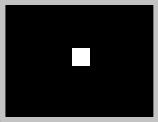
\includegraphics[width=0.48\textwidth]{single_graphic.png}
		\caption{The states of a single graphic stimulus.}
	\end{subfigure}
	~
	\begin{subfigure}{0.48\textwidth}
		
\includegraphics[width=0.48\textwidth]{pattern_reversal1.png}
		~
		
\includegraphics[width=0.48\textwidth]{pattern_reversal2.png}
		\caption{The states of a pattern reversal stimulus.}
	\end{subfigure}
	\caption{Different types of visual stimuli. A stimulus alternates between the two given states.}
	\label{fig:stimuli}
\end{figure}

The main difference between \gls{single graphic} stimuli and \gls{pattern reversal} stimuli is that \gls{single graphic} stimuli elicits \gls{SSVEP} response after every two alterations, while \gls{pattern reversal} stimuli elicits \gls{SSVEP} response after every alteration~\cite{ssvep_stim}. The fastest possible target frequency can be achieved by changing between the \glspl{state} of a target every time a new \gls{frame} is displayed. If the \gls{state} is changed at lower rate, the \gls{target} frequency will also be lower. Perhaps it is most reasonable to calculate the \gls{target} frequency with:
\begin{equation}
	f_{single\mbox{ }graphic} = \frac{n}{2T} \qquad f_{pattern\mbox{ }reversal} = \frac{n}{T}
\end{equation}
where $T$ is the period of the \gls{flickering waveform}, $n$ is the number of times the \gls{target} \gls{state} is switched in a time period of $T$ and $f$ is the \gls{flickering} frequency.

A computer monitor can be used to present visual stimuli to a subject and the \gls{refresh rate} of the monitor should be used for measuring the time between stimuli presentations. Adjusting \gls{target} \gls{flickering} to the rate at which the \glspl{frame} are changed can produce different \glspl{flickering waveform} for different \gls{flickering} frequencies. Since the \glspl{flickering waveform} are different, the \gls{SSVEP} responses are also different.

\section{Overview of Fourier analysis}
\label{sec:fourier}

As discussed in the previous section, the \gls{flickering} of a \gls{target} can produce different waveforms. This section will discuss how these waveforms and other signals can be represented by sums of simpler trigonometric functions. The study of this decomposition process is called Fourier analysis, named after Joseph Fourier, whose insight to model all functions by trigonometric series was a breakthrough in the field in 1807.

The following paragraph is based on the book by Hartmann~\cite{pure_tone}. The simpler trigonometric functions that a signal is decomposed into are \glspl{pure tone}---the waveforms that contain only one frequency. All other waveforms contain at least two frequencies. \Gls{pure tone} waveforms are sine and cosine waves. Important property of a \gls{pure tone} is that linear operations do not change the shape of the \gls{pure tone} waveform. See figure~\ref{fig:pure_tone} for an example of a \gls{pure tone}.

The \glspl{pure tone} are used to represent all possible frequencies that a signal may contain. The decomposition process of a signal is called \gls{Fourier transform} and it is used to decompose a function of time into \glspl{pure tone} or \glspl{frequency component} that make it up. The function of time can be for example the \gls{EEG} recording represented as voltage versus time or the \gls{target} \gls{flickering} represented as \gls{state} versus time. \Gls{Fourier transform} converts signal from time domain or the function of time to frequency domain or the function of frequency. The representation of a time-domain signal in a frequency domain is called \gls{frequency spectrum}. \Gls{frequency spectrum} contains information about amplitude and phase of different \glspl{frequency component}. Therefore, \gls{frequency spectrum} can be presented as a function of frequency versus amplitude and phase.

\begin{figure}[h]
	% This file was created by matplotlib v0.1.0.
% Copyright (c) 2010--2014, Nico Schlömer <nico.schloemer@gmail.com>
% All rights reserved.
% 
% The lastest updates can be retrieved from
% 
% https://github.com/nschloe/matplotlib2tikz
% 
% where you can also submit bug reports and leavecomments.
% 
\begin{tikzpicture}[scale=0.9]

\begin{groupplot}[group style={group size=2 by 1, horizontal sep=50pt}]
\nextgroupplot[
xmin=0, xmax=2,
ymin=-1, ymax=1,
axis on top,
xlabel = Time,
ylabel = Signal,
ylabel shift = -10 pt,
enlarge x limits = 0.1,
enlarge y limits = 0.1,
auto title
]
\addplot [blue, mark=*]
coordinates {
(0,4.44089209850063e-16)
(0.0512820512820513,0.316667993801473)
(0.102564102564103,0.600742264237979)
(0.153846153846154,0.822983865893657)
(0.205128205128205,0.960518111631373)
(0.256410256410256,0.99918899817157)
(0.307692307692308,0.935016242685415)
(0.358974358974359,0.774604961827655)
(0.41025641025641,0.534465826127802)
(0.461538461538462,0.239315664287559)
(0.512820512820513,-0.0804665687167249)
(0.564102564102564,-0.391966609860074)
(0.615384615384615,-0.663122658240795)
(0.666666666666667,-0.866025403784438)
(0.717948717948718,-0.979790652042267)
(0.769230769230769,-0.992708874098054)
(0.82051282051282,-0.903450434610382)
(0.871794871794872,-0.721202447343814)
(0.923076923076923,-0.464723172043769)
(0.974358974358974,-0.16041128085776)
(1.02564102564103,0.16041128085776)
(1.07692307692308,0.464723172043768)
(1.12820512820513,0.721202447343815)
(1.17948717948718,0.903450434610383)
(1.23076923076923,0.992708874098054)
(1.28205128205128,0.979790652042268)
(1.33333333333333,0.86602540378444)
(1.38461538461538,0.663122658240796)
(1.43589743589744,0.391966609860076)
(1.48717948717949,0.0804665687167263)
(1.53846153846154,-0.239315664287556)
(1.58974358974359,-0.5344658261278)
(1.64102564102564,-0.774604961827654)
(1.69230769230769,-0.935016242685414)
(1.74358974358974,-0.999188998171569)
(1.79487179487179,-0.960518111631372)
(1.84615384615385,-0.822983865893657)
(1.8974358974359,-0.600742264237979)
(1.94871794871795,-0.316667993801473)
(2,-4.57695098088787e-17)

};
\path [draw=black, fill opacity=0] (axis cs:13,1)--(axis cs:13,1);

\path [draw=black, fill opacity=0] (axis cs:2,13)--(axis cs:2,13);

\path [draw=black, fill opacity=0] (axis cs:13,-1)--(axis cs:13,-1);

\path [draw=black, fill opacity=0] (axis cs:0,13)--(axis cs:0,13);

\nextgroupplot[
xmin=0, xmax=10,
ymin=0, ymax=1,
axis on top,
xlabel = Frequency,
ylabel = Amplitude,
enlarge x limits = 0.1,
enlarge y limits = 0.1,
auto title
]
\addplot [blue, mark=*]
coordinates {
(0.5,0.0317296035410643)
(1,0.982863625528606)
(1.5,0.0642488968474364)
(2,0.0350688715308441)
(2.5,0.0250970809482021)
(3,0.0199256807572927)
(3.5,0.016728331802113)
(4,0.0145525501480966)
(4.5,0.0129818771154998)
(5,0.0118033464977954)
(5.5,0.0108960439627206)
(6,0.0101860398596371)
(6.5,0.00962562080824836)
(7,0.0091827528549743)
(7.5,0.00883532979770986)
(8,0.00856785212850308)
(8.5,0.00836942755874022)
(9,0.0082325343426935)
(9.5,0.008152251094645)
(10,0.0081257909009141)

};
\path [draw=black, fill opacity=0] (axis cs:13,20)--(axis cs:13,20);

\path [draw=black, fill opacity=0] (axis cs:10,13)--(axis cs:10,13);

\path [draw=black, fill opacity=0] (axis cs:13,0)--(axis cs:13,0);

\path [draw=black, fill opacity=0] (axis cs:0,13)--(axis cs:0,13);

\end{groupplot}

\end{tikzpicture}
	\caption{A sine wave in time domain~(A) and its frequency components' amplitudes~(B). Theoretically pure tone has only one frequency, but since the signal in time domain is digital, it is an approximation of the actual pure tone and therefore the representation of frequency components' amplitudes is not perfect.}
	\label{fig:pure_tone}
\end{figure}

To represent both amplitude and phase, complex numbers are used. Complex numbers can be represented as a pair of real numbers and therefore complex numbers can be used to represent two values. The amplitude and phase do not correspond to the real and imaginary part of the complex number but rather are related to the absolute value or the modulus and the phase of the complex number. In this thesis the phase information from the \gls{frequency spectrum} is not used. There are, however, \glspl{BCI} that also use the phase information~\cite{MPCC}. Since only the information about amplitude is required in this thesis, it is possible to convert the \gls{frequency spectrum} into \gls{power spectral density}, which can be represented as a function of amplitude squared or power versus frequency.

To conclude previous discussion, the amount of frequency $f$ present in a signal can be calculated by first calculating the \gls{frequency spectrum} with \gls{Fourier transform} and then taking modulus squared of the \gls{frequency spectrum}'s value at frequency $f$.

In digital devices, however, theoretical \gls{power spectral density} cannot be calculated. The measurement period would have to be infinitely long to a acquire the true \gls{power spectral density}~\cite{psd}. Therefore, spectral estimation is used. The modulus squared of frequency spectrum in a real-world application is called \gls{periodogram} and it is the estimation of the \gls{power spectral density}. There are other spectral estimation methods available.

Since digital devices work with \glspl{digital signal} as discussed in section~\ref{sec:EEG_comparison}, in a real-world application discrete version of the \gls{Fourier transform} is used. The algorithm used to compute the discrete \gls{Fourier transform} is called \gls{FFT}. The \gls{frequency spectrum} calculated by \gls{FFT} is discrete---if the digital real-valued input signal, as is the case with \gls{EEG} recording, has $N$ values then the output has the integer part of $\frac{N}{2}$ values. This derives from the definition and symmetric property of the discrete \gls{Fourier transform}. %The higher the sampling rate and \gls{ADC} resolution of a recording device, the more accurate the recording and therefore the more accurate the frequency spectrum and the periodogram of the signal.

The signal that is recorded, however, may contain frequencies that are too high to be detected from the \gls{digital signal}. Theoretically, the \gls{sampling rate} of the device has to be more than two times higher than the highest frequency in the signal to reconstruct the continuous signal from the recorded \gls{digital signal} and also to decompose the signal into \glspl{frequency component}. The highest frequency that can be detected with a \gls{sampling rate} of $f$ is $\frac{2}{f}$ and it is called \gls{Nyguist frequency}. But since real-world application are imperfect, even higher \gls{sampling rate} is needed. For example, as discussed in section~\ref{sec:EEG_comparison}, Emotiv EPOC has internal \gls{sampling rate} of \SI{2048}{Hz} to more accurately record frequencies up to its \gls{Nyguist frequency} of $\frac{\SI{128}{Hz}}{2}=\SI{64}{Hz}$, since the actual \gls{sampling rate} is \SI{128}{Hz}.

To conclude previous discussion, the \gls{frequency spectrum} calculated by \gls{FFT} from real-valued time-domain signal with $N$ values is defined at frequencies $\frac{1}{N}, \frac{2}{N}, \dots\frac{f/2}{N}$. These frequencies are also called \glspl{frequency bin}. The length of a \gls{frequency spectrum} depends on the length of the signal from which it is calculated. The longer the input signal, the more \glspl{frequency bin} will be acquired.

Thus a time-domain signal can be decomposed into \glspl{pure tone} or sine and cosine waves using \gls{FFT}. \gls{FFT} calculates the \gls{frequency spectrum} of a time-domain signal. \Gls{frequency spectrum} can be converted to the estimation of \gls{power spectral density} which contains only the information about the amplitudes of the \glspl{pure tone}. Analysing the \gls{power spectral density} can be used to detect \glspl{SSVEP} in an \gls{EEG} recording.

%As already discussed in section~\ref{sec:EEG_comparison}, Emotiv EPOC has high internal sampling rate to filter out high frequencies

%Thus higher sampling rate and \gls{ADC} resolution lead to more accurate \gls{SSVEP} detection.

\section{Decomposing target flickering}
\label{sec:decomposition}

This section will focus on the decomposition of the \glspl{flickering waveform}, which were described in section~\ref{sec:stimuli}. The decomposition process was discussed in section~\ref{sec:fourier}. As discussed in previous section, only sine and cosine waves are composed of a single frequency. Other waveforms have more \glspl{frequency component}.

The \gls{frequency component} of a signal that has the lowest frequency among all the \glspl{frequency component} of the signal is called \gls{fundamental} or the first \gls{harmonic} of the signal. \Gls{harmonic} of a signal is a \gls{frequency component} with frequency that is an integer multiple of the \gls{fundamental} frequency of the signal. If the \gls{fundamental} frequency is $f$, then first, second are third \glspl{harmonic} have frequencies of $1f$, $2f$, $3f$ respectively.

It can be shown that a \gls{square wave} is composed of its odd \glspl{harmonic}. If the \gls{flickering waveform} is a \gls{square wave} or a \gls{rectangular wave}, the \gls{fundamental} frequency of the waveform is the frequency of the stimuli presentation. Therefore, a \gls{square wave} with \gls{fundamental} frequency $f$ can be represented as a sum of sine waves
\begin{equation}
	\label{eq:square}
	\mbox{square}(t) = \sum_{n=1,3,5,\dots}^{\infty}\frac{1}{n} \sin(2\pi nft)
\end{equation}
where $\mbox{square}(t)$ is the \gls{flickering} represented as \gls{state} versus time, $\frac{1}{n}$ is the amplitude of a \gls{frequency component} and $f$ is the \gls{fundamental} frequency of the waveform. See figure~\ref{fig:square_wave} for an example of a \gls{square wave}, three of its \glspl{harmonic} and their amplitude spectrum. It can be seen that the \gls{fundamental} of the square wave has the highest amplitude among its \glspl{frequency component}. \Gls{rectangular wave}'s \glspl{frequency component} depend on the \gls{duty cycle} of the wave. But as is the case with \glspl{square wave}, the \gls{fundamental} has the highest amplitude also in a \gls{rectangular wave}.

\begin{figure}[h]
	% This file was created by matplotlib v0.1.0.
% Copyright (c) 2010--2014, Nico Schlömer <nico.schloemer@gmail.com>
% All rights reserved.
% 
% The lastest updates can be retrieved from
% 
% https://github.com/nschloe/matplotlib2tikz
% 
% where you can also submit bug reports and leavecomments.
% 
\begin{tikzpicture}[scale=0.9]

\begin{groupplot}[group style={group size=2 by 1, horizontal sep=50pt}]
\nextgroupplot[
xmin=0, xmax=2,
ymin=-1.5, ymax=1.5,
axis on top,
xlabel = Time,
ylabel = Signal,
ylabel shift = -10 pt,
enlarge x limits = 0.05,
enlarge y limits = 0.05,
auto title
]
\addplot [blue]
coordinates {
(0,4.44089209850063e-16)
(0.0253164556962025,0.158398024407215)
(0.0506329113924051,0.312796607022228)
(0.0759493670886076,0.459297289222978)
(0.10126582278481,0.594201028971711)
(0.126582278481013,0.71410159909675)
(0.151898734177215,0.815971592199161)
(0.177215189873418,0.897238860619213)
(0.20253164556962,0.955851461405761)
(0.227848101265823,0.990329466472502)
(0.253164556962025,0.999802329770066)
(0.278481012658228,0.984030867978421)
(0.30379746835443,0.943413299722135)
(0.329113924050633,0.878975190822434)
(0.354430379746835,0.792343559461575)
(0.379746835443038,0.685705795086414)
(0.405063291139241,0.561754428320772)
(0.430379746835443,0.423619146408528)
(0.455696202531646,0.274787770751026)
(0.481012658227848,0.119018191801905)
(0.506329113924051,-0.0397565150969252)
(0.531645569620253,-0.197527397177952)
(0.556962025316456,-0.350310847563824)
(0.582278481012658,-0.494249188616722)
(0.607594936708861,-0.625708075660559)
(0.632911392405063,-0.741368261698618)
(0.658227848101266,-0.838309406130276)
(0.683544303797468,-0.914083811354034)
(0.708860759493671,-0.966778225458037)
(0.734177215189873,-0.995062150522427)
(0.759493670886076,-0.998221436781933)
(0.784810126582278,-0.976176314419051)
(0.810126582278481,-0.929483407697387)
(0.835443037974684,-0.859321680579661)
(0.860759493670886,-0.767462668693907)
(0.886075949367089,-0.656225749270376)
(0.911392405063291,-0.528419578452619)
(0.936708860759494,-0.387271174650641)
(0.962025316455696,-0.236344438532905)
(0.987341772151899,-0.0794501669717144)
(1.0126582278481,0.0794501669717148)
(1.0379746835443,0.236344438532905)
(1.06329113924051,0.387271174650641)
(1.08860759493671,0.52841957845262)
(1.11392405063291,0.656225749270376)
(1.13924050632911,0.767462668693908)
(1.16455696202532,0.859321680579661)
(1.18987341772152,0.929483407697387)
(1.21518987341772,0.976176314419051)
(1.24050632911392,0.998221436781933)
(1.26582278481013,0.995062150522428)
(1.29113924050633,0.966778225458038)
(1.31645569620253,0.914083811354035)
(1.34177215189873,0.838309406130277)
(1.36708860759494,0.74136826169862)
(1.39240506329114,0.625708075660561)
(1.41772151898734,0.494249188616724)
(1.44303797468354,0.350310847563826)
(1.46835443037975,0.197527397177952)
(1.49367088607595,0.0397565150969266)
(1.51898734177215,-0.119018191801903)
(1.54430379746835,-0.274787770751025)
(1.56962025316456,-0.423619146408527)
(1.59493670886076,-0.56175442832077)
(1.62025316455696,-0.685705795086412)
(1.64556962025316,-0.792343559461573)
(1.67088607594937,-0.878975190822433)
(1.69620253164557,-0.943413299722134)
(1.72151898734177,-0.98403086797842)
(1.74683544303797,-0.999802329770065)
(1.77215189873418,-0.990329466472502)
(1.79746835443038,-0.95585146140576)
(1.82278481012658,-0.897238860619212)
(1.84810126582278,-0.815971592199161)
(1.87341772151899,-0.71410159909675)
(1.89873417721519,-0.594201028971711)
(1.92405063291139,-0.459297289222978)
(1.94936708860759,-0.312796607022228)
(1.9746835443038,-0.158398024407216)
(2,-4.57695098088787e-17)

};
\addplot [green!50.0!black]
coordinates {
(0,4.44089209850063e-16)
(0.0253164556962025,0.311497120814875)
(0.0506329113924051,0.584787137755281)
(0.0759493670886076,0.789407111380479)
(0.10126582278481,0.908672128879089)
(0.126582278481013,0.942670197458888)
(0.151898734177215,0.907567515782837)
(0.177215189873418,0.831396394893229)
(0.20253164556962,0.747282102852241)
(0.227848101265823,0.685634862687824)
(0.253164556962025,0.667061850842755)
(0.278481012658228,0.697590307785201)
(0.30379746835443,0.767273440237928)
(0.329113924050633,0.852491801831863)
(0.354430379746835,0.921433951011788)
(0.379746835443038,0.94152668465105)
(0.405063291139241,0.887146533127122)
(0.430379746835443,0.745878554894541)
(0.455696202531646,0.521910524650565)
(0.481012658227848,0.23578847432318)
(0.506329113924051,-0.0794292456975601)
(0.531645569620253,-0.384778873284875)
(0.556962025316456,-0.643302577837968)
(0.582278481012658,-0.827516631873411)
(0.607594936708861,-0.924787695866964)
(0.632911392405063,-0.939435271355854)
(0.658227848101266,-0.891108747599348)
(0.683544303797468,-0.809818275679959)
(0.708860759493671,-0.728744359092454)
(0.734177215189873,-0.676444996720507)
(0.759493670886076,-0.670211147455792)
(0.784810126582278,-0.712061794598526)
(0.810126582278481,-0.78827702556121)
(0.835443037974684,-0.872573852278636)
(0.860759493670886,-0.932212398232815)
(0.886075949367089,-0.935662217980468)
(0.911392405063291,-0.860106961960095)
(0.936708860759494,-0.697098977216437)
(0.962025316455696,-0.455086354956363)
(0.987341772151899,-0.158231646482683)
(1.0126582278481,0.158231646482683)
(1.0379746835443,0.455086354956363)
(1.06329113924051,0.697098977216436)
(1.08860759493671,0.860106961960096)
(1.11392405063291,0.935662217980468)
(1.13924050632911,0.932212398232816)
(1.16455696202532,0.872573852278637)
(1.18987341772152,0.788277025561212)
(1.21518987341772,0.712061794598527)
(1.24050632911392,0.670211147455793)
(1.26582278481013,0.676444996720508)
(1.29113924050633,0.728744359092454)
(1.31645569620253,0.809818275679959)
(1.34177215189873,0.891108747599349)
(1.36708860759494,0.939435271355855)
(1.39240506329114,0.924787695866965)
(1.41772151898734,0.827516631873412)
(1.44303797468354,0.643302577837972)
(1.46835443037975,0.384778873284876)
(1.49367088607595,0.079429245697562)
(1.51898734177215,-0.235788474323176)
(1.54430379746835,-0.521910524650565)
(1.56962025316456,-0.745878554894539)
(1.59493670886076,-0.88714653312712)
(1.62025316455696,-0.941526684651049)
(1.64556962025316,-0.921433951011788)
(1.67088607594937,-0.852491801831862)
(1.69620253164557,-0.767273440237929)
(1.72151898734177,-0.6975903077852)
(1.74683544303797,-0.667061850842754)
(1.77215189873418,-0.685634862687823)
(1.79746835443038,-0.74728210285224)
(1.82278481012658,-0.831396394893228)
(1.84810126582278,-0.907567515782837)
(1.87341772151899,-0.942670197458887)
(1.89873417721519,-0.908672128879089)
(1.92405063291139,-0.789407111380478)
(1.94936708860759,-0.584787137755283)
(1.9746835443038,-0.311497120814876)
(2,-5.3562822946782e-16)

};
\addplot [red]
coordinates {
(0,4.44089209850063e-16)
(0.0253164556962025,0.454317440634225)
(0.0506329113924051,0.784747603709294)
(0.0759493670886076,0.926548270397762)
(0.10126582278481,0.900720825859704)
(0.126582278481013,0.794396545119164)
(0.151898734177215,0.70792322842645)
(0.177215189873418,0.700151245039153)
(0.20253164556962,0.763172136246584)
(0.227848101265823,0.839127396426606)
(0.253164556962025,0.86607428094724)
(0.278481012658228,0.822731922917313)
(0.30379746835443,0.743469801877548)
(0.329113924050633,0.694023089939548)
(0.354430379746835,0.723368057717288)
(0.379746835443038,0.822686478856707)
(0.405063291139241,0.918826138008564)
(0.430379746835443,0.909072873334373)
(0.455696202531646,0.718716698246249)
(0.481012658227848,0.348139359987334)
(0.506329113924051,-0.118934725133151)
(0.531645569620253,-0.55244075451093)
(0.556962025316456,-0.838537840721778)
(0.582278481012658,-0.933200547563935)
(0.607594936708861,-0.877518808160383)
(0.632911392405063,-0.767570935239922)
(0.658227848101266,-0.69775310250774)
(0.683544303797468,-0.710968437956614)
(0.708860759493671,-0.783701913242659)
(0.734177215189873,-0.852240034884994)
(0.759493670886076,-0.861381439736945)
(0.784810126582278,-0.803921252443122)
(0.810126582278481,-0.725717704156766)
(0.835443037974684,-0.693126080154793)
(0.860759493670886,-0.743529738288388)
(0.886075949367089,-0.850938388698761)
(0.911392405063291,-0.930169131472859)
(0.936708860759494,-0.879915739487244)
(0.962025316455696,-0.640983036495841)
(0.987341772151899,-0.235685881412812)
(1.0126582278481,0.235685881412811)
(1.0379746835443,0.64098303649584)
(1.06329113924051,0.879915739487243)
(1.08860759493671,0.93016913147286)
(1.11392405063291,0.850938388698763)
(1.13924050632911,0.743529738288389)
(1.16455696202532,0.693126080154794)
(1.18987341772152,0.725717704156766)
(1.21518987341772,0.803921252443122)
(1.24050632911392,0.861381439736945)
(1.26582278481013,0.852240034884995)
(1.29113924050633,0.78370191324266)
(1.31645569620253,0.710968437956615)
(1.34177215189873,0.697753102507741)
(1.36708860759494,0.767570935239922)
(1.39240506329114,0.877518808160383)
(1.41772151898734,0.933200547563936)
(1.44303797468354,0.838537840721782)
(1.46835443037975,0.552440754510931)
(1.49367088607595,0.118934725133152)
(1.51898734177215,-0.348139359987329)
(1.54430379746835,-0.71871669824625)
(1.56962025316456,-0.909072873334372)
(1.59493670886076,-0.918826138008564)
(1.62025316455696,-0.822686478856708)
(1.64556962025316,-0.723368057717288)
(1.67088607594937,-0.694023089939547)
(1.69620253164557,-0.743469801877547)
(1.72151898734177,-0.822731922917312)
(1.74683544303797,-0.86607428094724)
(1.77215189873418,-0.839127396426606)
(1.79746835443038,-0.763172136246582)
(1.82278481012658,-0.700151245039154)
(1.84810126582278,-0.70792322842645)
(1.87341772151899,-0.794396545119163)
(1.89873417721519,-0.900720825859703)
(1.92405063291139,-0.92654827039776)
(1.94936708860759,-0.784747603709296)
(1.9746835443038,-0.454317440634226)
(2,-1.02548694912676e-15)

};
\addplot [black, thick]
coordinates {
(0,0.785398163397449)
(0.0253164556962025,0.785398163397449)
(0.0506329113924051,0.785398163397449)
(0.0759493670886076,0.785398163397449)
(0.10126582278481,0.785398163397449)
(0.126582278481013,0.785398163397449)
(0.151898734177215,0.785398163397449)
(0.177215189873418,0.785398163397449)
(0.20253164556962,0.785398163397449)
(0.227848101265823,0.785398163397449)
(0.253164556962025,0.785398163397449)
(0.278481012658228,0.785398163397449)
(0.30379746835443,0.785398163397449)
(0.329113924050633,0.785398163397449)
(0.354430379746835,0.785398163397449)
(0.379746835443038,0.785398163397449)
(0.405063291139241,0.785398163397449)
(0.430379746835443,0.785398163397449)
(0.455696202531646,0.785398163397449)
(0.481012658227848,0.785398163397449)
(0.506329113924051,-0.785398163397448)
(0.531645569620253,-0.785398163397448)
(0.556962025316456,-0.785398163397448)
(0.582278481012658,-0.785398163397448)
(0.607594936708861,-0.785398163397448)
(0.632911392405063,-0.785398163397448)
(0.658227848101266,-0.785398163397448)
(0.683544303797468,-0.785398163397448)
(0.708860759493671,-0.785398163397448)
(0.734177215189873,-0.785398163397448)
(0.759493670886076,-0.785398163397448)
(0.784810126582278,-0.785398163397448)
(0.810126582278481,-0.785398163397448)
(0.835443037974684,-0.785398163397448)
(0.860759493670886,-0.785398163397448)
(0.886075949367089,-0.785398163397448)
(0.911392405063291,-0.785398163397448)
(0.936708860759494,-0.785398163397448)
(0.962025316455696,-0.785398163397448)
(0.987341772151899,-0.785398163397448)
(1.0126582278481,0.785398163397449)
(1.0379746835443,0.785398163397449)
(1.06329113924051,0.785398163397449)
(1.08860759493671,0.785398163397449)
(1.11392405063291,0.785398163397449)
(1.13924050632911,0.785398163397449)
(1.16455696202532,0.785398163397449)
(1.18987341772152,0.785398163397449)
(1.21518987341772,0.785398163397449)
(1.24050632911392,0.785398163397449)
(1.26582278481013,0.785398163397449)
(1.29113924050633,0.785398163397449)
(1.31645569620253,0.785398163397449)
(1.34177215189873,0.785398163397449)
(1.36708860759494,0.785398163397449)
(1.39240506329114,0.785398163397449)
(1.41772151898734,0.785398163397449)
(1.44303797468354,0.785398163397449)
(1.46835443037975,0.785398163397449)
(1.49367088607595,0.785398163397449)
(1.51898734177215,-0.785398163397448)
(1.54430379746835,-0.785398163397448)
(1.56962025316456,-0.785398163397448)
(1.59493670886076,-0.785398163397448)
(1.62025316455696,-0.785398163397448)
(1.64556962025316,-0.785398163397448)
(1.67088607594937,-0.785398163397448)
(1.69620253164557,-0.785398163397448)
(1.72151898734177,-0.785398163397448)
(1.74683544303797,-0.785398163397448)
(1.77215189873418,-0.785398163397448)
(1.79746835443038,-0.785398163397448)
(1.82278481012658,-0.785398163397448)
(1.84810126582278,-0.785398163397448)
(1.87341772151899,-0.785398163397448)
(1.89873417721519,-0.785398163397448)
(1.92405063291139,-0.785398163397448)
(1.94936708860759,-0.785398163397448)
(1.9746835443038,-0.785398163397448)
(2,0.785398163397449)

};
\path [draw=black, fill opacity=0] (axis cs:13,1)--(axis cs:13,1);

\path [draw=black, fill opacity=0] (axis cs:2,13)--(axis cs:2,13);

\path [draw=black, fill opacity=0] (axis cs:13,-1)--(axis cs:13,-1);

\path [draw=black, fill opacity=0] (axis cs:0,13)--(axis cs:0,13);


\nextgroupplot[
xmin=0, xmax=20,
ymin=0, ymax=1,
axis on top,
xlabel = Frequency,
ylabel = Amplitude,
enlarge x limits = 0.05,
enlarge y limits = 0.05,
auto title
]

\addplot [black, mark=*]
coordinates {
(6,0.0295455422582101)
(6.5,0.0392699081698724)
(7,0.0392699081698724)
(7.5,0.134046551478503)
(8,0.0392699081698724)
(8.5,0.0392699081698725)
(9,0.0392699081698724)
(9.5,0.0999922819240693)
(10,0.0392699081698724)
(10.5,0.0392699081698724)
(11,0.0392699081698724)
(11.5,0.0777287820956132)
(12,0.0392699081698724)
(12.5,0.0392699081698724)
(13,0.0392699081698724)
(13.5,0.0621172398460391)
(14,0.0392699081698723)
(14.5,0.0392699081698724)
(15,0.0392699081698724)
(15.5,0.0509948373917945)
(16,0.0392699081698724)
(16.5,0.0392699081698724)
(17,0.0392699081698724)
(17.5,0.0435621932489829)
(18,0.0392699081698724)
(18.5,0.0392699081698724)
(19,0.0392699081698724)
(19.5,0.0397534041144176)
(20,0.0392699081698724)

};

\addplot [red, mark=*]
coordinates {
(4,0.0291487323922272)
(4.5,0.0101247851443722)
(5,0.0204727312731035)
(5.5,0.193408492248942)
(6,0.0295455422582101)

};
\addplot [blue, mark=*]
coordinates {
(1,0.016292922345932)
(1.5,0.992637301349993)
(2,0.0310182748004185)
(2.5,0.00953818939550112)

};
\addplot [green!50.0!black, mark=*]
coordinates {
(2.5,0.00953818939550112)
(3,0.0209766408288386)
(3.5,0.328023460602311)
(4,0.0291487323922272)

};
\path [draw=black, fill opacity=0] (axis cs:13,70)--(axis cs:13,70);

\path [draw=black, fill opacity=0] (axis cs:25,13)--(axis cs:25,13);

\path [draw=black, fill opacity=0] (axis cs:13,0)--(axis cs:13,0);

\path [draw=black, fill opacity=0] (axis cs:0,13)--(axis cs:0,13);

\end{groupplot}

\end{tikzpicture}
	\caption{A square wave in time domain (A), its first harmonic (blue), the sum of its first two harmonics (green) and the sum of its first three harmonics (red). The amplitude spectrum (B) shows the amplitudes of the same signals with the same colour-coding. Please note that the green signal also contains the blue signal, the red signal contains both blue and green signal and black signal contains all the previous signals. In general, every next signal in amplitude spectrum also contains the previous signals.}
	\label{fig:square_wave}
\end{figure}

Unfortunately, the \gls{SSVEP} response to \gls{target} \gls{flickering} does not contain only the frequencies that are present in the \glspl{frequency component} of the \gls{flickering waveform}---\gls{SSVEP} contains other frequencies too. However, the frequencies that are present in the \glspl{frequency component} of the \gls{flickering waveform} are more successfully elicited in \gls{SSVEP} response~\cite{square_sine}.

Generally an \gls{SSVEP} contains \glspl{frequency component} with frequencies that are integer multiples of the \gls{flickering} frequency~\cite{ssvep_response}. Therefore, \gls{target} frequencies should be chosen so that neither of these frequencies is an integer multiple of the other. Otherwise it might not be distinguishable which \gls{target} \gls{flickering} elicits which frequency in the \gls{SSVEP} response. For example, if \SI{6}{Hz} and \SI{12}{Hz} Hz \gls{flickering} frequencies are both used, then \SI{6}{Hz} \gls{flickering} also elicits \SI{12}{Hz} frequency in the \gls{SSVEP} since \SI{12}{Hz} is the second harmonic of \SI{6}{Hz} \gls{flickering} and thus it might not be possible to distinguish this \SI{12}{Hz} component from the \SI{12}{Hz} component elicited by \SI{12}{Hz} \gls{flickering}.

It has even been reported that \gls{SSVEP} contains \glspl{frequency component} that have lower frequency than the \gls{fundamental} of the \gls{flickering waveform}~\cite{ssvep_response}. These \glspl{frequency component} have frequency of $\frac{f}{n}$, where $f$ is the \gls{fundamental} frequency of the \gls{flickering waveform} and $n$ is a natural number. But since these components have very small amplitudes, these components are not used in \gls{SSVEP}-based \glspl{BCI}.

An \gls{SSVEP} reflects certain properties of the visual stimulus. The frequencies that are present in the \gls{flickering waveform} are likely to be found also in the \gls{SSVEP} response, but other \glspl{frequency component} are present in the \gls{SSVEP} too~\cite{square_sine}. It is sufficient to detect only the \gls{frequency component} with the same frequency as the \gls{target} \gls{flickering} in a \gls{SSVEP}-based \gls{BCI}, but to improve the performance of the \gls{BCI} other \glspl{frequency component} should be detected too~\cite{harmonic_imrpovement}.

%Most important of these properties is that \gls{SSVEP} has a component with the same frequency as the visual stimulus. But that is not the only component frequency in \gls{SSVEP}. \gls{SSVEP} has other components too that are discussed in section~\ref{sec:fourier}. 

\section{Evaluating the performance of a brain-computer interface}

The most commonly used method for evaluating the performance of a \gls{BCI} is called \gls{ITR}~\cite{itr}. \gls{ITR} was defined by Wolpaw \textit{et al.}~\cite{itr_wolpaw} in 1998
\begin{equation}
	\label{eq:itr_unit}
	B=\log_2 N+ P\log_2 P +(1-P)\log_2[(1-P)/(N-1)]
\end{equation}
where $B$ is the \gls{ITR} in units of bits per trial or bits per command, $N$ is the number of targets and $P$ is the accuracy or the probability that the user's choice is actually selected. To make the units of \gls{ITR} more understandable, \gls{ITR} is calculated in units of bits per minute~\cite{itr_wolpaw}
\begin{equation}
	\label{eq:itr}
	B_t=B\cdot(\frac{60}{T})
\end{equation}
where $B_t$ is the \gls{ITR}, $B$ is calculated with equation~\ref{eq:itr_unit} and $T$ is the time needed to identify a chosen command.

There are, however, preconditions that have to be fulfilled in order to calculate correct \gls{ITR} with the previously given equations. These preconditions are the following: \gls{BCI} is memoryless, all commands are equally likely to be chosen, the accuracy of choosing a target is the same for every target and in case of choosing a wrong target, all wrong targets are equally likely to he chosen~\cite{itr}.

If these preconditions are met, the \gls{ITR} of a \gls{BCI} can be calculated using equation~\ref{eq:itr}. Using the same evaluation method allows the performance of different \glspl{BCI} to be easily compared.

\section{Improving the accuracy of a spectrum with signal processing}
\label{sec:signal_processing}

The aim of this section is to describe some digital signal processing techniques that can improve the performance of a \gls{SSVEP}-based \gls{BCI} by improving the accuracy of an amplitude spectrum or \gls{power spectral density}.

\subsection{Detrending the signal}
\label{sec:detrend}

A linear \gls{trend} or steady increase or decrease of values in an \gls{EEG} recording can make the detection of \glspl{SSVEP} less accurate. As discussed in section~\ref{sec:fourier}, \gls{Fourier transform} is used to decompose a signal into \glspl{frequency component}. If the signal has a \gls{trend}, the \gls{trend} will also be decomposed. The decomposed \gls{trend} will not provide any useful information and it makes detecting the actual \gls{SSVEP} less accurate. A comparison of amplitudes acquired from a signal with trend and from the same signal without \gls{trend} can be seen in figure~\ref{fig:detrend}.

\begin{figure}[h!]
	% This file was created by matplotlib v0.1.0.
% Copyright (c) 2010--2014, Nico Schlömer <nico.schloemer@gmail.com>
% All rights reserved.
% 
% The lastest updates can be retrieved from
% 
% https://github.com/nschloe/matplotlib2tikz
% 
% where you can also submit bug reports and leavecomments.
% 
\begin{tikzpicture}[scale=0.9]

\begin{groupplot}[group style={group size=2 by 2, horizontal sep=50pt}]
\nextgroupplot[
xmin=0, xmax=3,
ymin=-2, ymax=4,
axis on top,
ylabel = Signal,
ylabel shift = -10 pt,
enlarge x limits = 0.05,
enlarge y limits = 0.05
]
\addplot [blue]
coordinates {
(0,-3.5527136788005e-15)
(0.0769230769230769,0.541646248966842)
(0.153846153846154,0.976830019739807)
(0.230769230769231,1.22347810486728)
(0.307692307692308,1.24270855037772)
(0.384615384615385,1.04773804285618)
(0.461538461538462,0.700854125826016)
(0.538461538461538,0.299145874173977)
(0.615384615384615,-0.0477380428561834)
(0.692307692307692,-0.242708550377726)
(0.769230769230769,-0.223478104867288)
(0.846153846153846,0.0231699802601867)
(0.923076923076923,0.458353751033151)
(1,0.999999999999996)
(1.07692307692308,1.54164624896684)
(1.15384615384615,1.97683001973981)
(1.23076923076923,2.22347810486728)
(1.30769230769231,2.24270855037772)
(1.38461538461538,2.04773804285618)
(1.46153846153846,1.70085412582601)
(1.53846153846154,1.29914587417398)
(1.61538461538462,0.952261957143817)
(1.69230769230769,0.757291449622273)
(1.76923076923077,0.776521895132712)
(1.84615384615385,1.02316998026019)
(1.92307692307692,1.45835375103315)
(2,2)
(2.07692307692308,2.54164624896684)
(2.15384615384615,2.97683001973981)
(2.23076923076923,3.22347810486728)
(2.30769230769231,3.24270855037772)
(2.38461538461538,3.04773804285618)
(2.46153846153846,2.70085412582602)
(2.53846153846154,2.29914587417398)
(2.61538461538461,1.95226195714382)
(2.69230769230769,1.75729144962227)
(2.76923076923077,1.77652189513271)
(2.84615384615385,2.02316998026019)
(2.92307692307692,2.45835375103315)
(3,3)

};
\addplot [black]
coordinates {
(0,-3.5527136788005e-15)
(0.0769230769230769,0.0769230769230734)
(0.153846153846154,0.15384615384615)
(0.230769230769231,0.230769230769227)
(0.307692307692308,0.307692307692304)
(0.384615384615385,0.384615384615381)
(0.461538461538462,0.461538461538458)
(0.538461538461538,0.538461538461535)
(0.615384615384615,0.615384615384612)
(0.692307692307692,0.692307692307689)
(0.769230769230769,0.769230769230765)
(0.846153846153846,0.846153846153842)
(0.923076923076923,0.923076923076919)
(1,0.999999999999996)
(1.07692307692308,1.07692307692307)
(1.15384615384615,1.15384615384615)
(1.23076923076923,1.23076923076923)
(1.30769230769231,1.3076923076923)
(1.38461538461538,1.38461538461538)
(1.46153846153846,1.46153846153846)
(1.53846153846154,1.53846153846153)
(1.61538461538462,1.61538461538461)
(1.69230769230769,1.69230769230769)
(1.76923076923077,1.76923076923077)
(1.84615384615385,1.84615384615384)
(1.92307692307692,1.92307692307692)
(2,2)
(2.07692307692308,2.07692307692307)
(2.15384615384615,2.15384615384615)
(2.23076923076923,2.23076923076923)
(2.30769230769231,2.3076923076923)
(2.38461538461538,2.38461538461538)
(2.46153846153846,2.46153846153846)
(2.53846153846154,2.53846153846153)
(2.61538461538461,2.61538461538461)
(2.69230769230769,2.69230769230769)
(2.76923076923077,2.76923076923077)
(2.84615384615385,2.84615384615384)
(2.92307692307692,2.92307692307692)
(3,3)

};
\addplot [green!50.0!black]
coordinates {
(0,-0.28944369501199)
(0.0769230769230769,0.190122743442649)
(0.153846153846154,0.563226703703408)
(0.230769230769231,0.747794978318677)
(0.307692307692308,0.704945613316909)
(0.384615384615385,0.447895295283161)
(0.461538461538462,0.0389315677407944)
(0.538461538461538,-0.42485649442345)
(0.615384615384615,-0.833820221965816)
(0.692307692307692,-1.09087053999956)
(0.769230769230769,-1.13371990500133)
(0.846153846153846,-0.949151630386063)
(0.923076923076923,-0.576047670125305)
(1,-0.0964812316706653)
(1.07692307692308,0.383085206783975)
(1.15384615384615,0.756189167044734)
(1.23076923076923,0.940757441660002)
(1.30769230769231,0.897908076658234)
(1.38461538461538,0.640857758624486)
(1.46153846153846,0.231894031082119)
(1.53846153846154,-0.231894031082125)
(1.61538461538462,-0.640857758624491)
(1.69230769230769,-0.89790807665824)
(1.76923076923077,-0.940757441660007)
(1.84615384615385,-0.756189167044738)
(1.92307692307692,-0.38308520678398)
(2,0.0964812316706593)
(2.07692307692308,0.5760476701253)
(2.15384615384615,0.949151630386061)
(2.23076923076923,1.13371990500133)
(2.30769230769231,1.09087053999956)
(2.38461538461538,0.833820221965812)
(2.46153846153846,0.424856494423444)
(2.53846153846154,-0.0389315677408009)
(2.61538461538461,-0.447895295283166)
(2.69230769230769,-0.704945613316914)
(2.76923076923077,-0.747794978318683)
(2.84615384615385,-0.563226703703413)
(2.92307692307692,-0.190122743442652)
(3,0.289443695011984)

};
\addplot [black]
coordinates {
(0,-3.5527136788005e-15)
(0.0769230769230769,-3.5527136788005e-15)
(0.153846153846154,-3.5527136788005e-15)
(0.230769230769231,-3.5527136788005e-15)
(0.307692307692308,-3.5527136788005e-15)
(0.384615384615385,-3.5527136788005e-15)
(0.461538461538462,-3.5527136788005e-15)
(0.538461538461538,-3.5527136788005e-15)
(0.615384615384615,-3.5527136788005e-15)
(0.692307692307692,-3.5527136788005e-15)
(0.769230769230769,-3.5527136788005e-15)
(0.846153846153846,-3.5527136788005e-15)
(0.923076923076923,-3.5527136788005e-15)
(1,-3.5527136788005e-15)
(1.07692307692308,-3.5527136788005e-15)
(1.15384615384615,-3.5527136788005e-15)
(1.23076923076923,-3.5527136788005e-15)
(1.30769230769231,-3.5527136788005e-15)
(1.38461538461538,-3.5527136788005e-15)
(1.46153846153846,-3.5527136788005e-15)
(1.53846153846154,-3.5527136788005e-15)
(1.61538461538462,-3.5527136788005e-15)
(1.69230769230769,-3.5527136788005e-15)
(1.76923076923077,-3.5527136788005e-15)
(1.84615384615385,-3.5527136788005e-15)
(1.92307692307692,-3.5527136788005e-15)
(2,-3.5527136788005e-15)
(2.07692307692308,-3.5527136788005e-15)
(2.15384615384615,-3.5527136788005e-15)
(2.23076923076923,-3.5527136788005e-15)
(2.30769230769231,-3.5527136788005e-15)
(2.38461538461538,-3.5527136788005e-15)
(2.46153846153846,-3.5527136788005e-15)
(2.53846153846154,-3.5527136788005e-15)
(2.61538461538461,-3.5527136788005e-15)
(2.69230769230769,-3.5527136788005e-15)
(2.76923076923077,-3.5527136788005e-15)
(2.84615384615385,-3.5527136788005e-15)
(2.92307692307692,-3.5527136788005e-15)
(3,-3.5527136788005e-15)

};
\path [draw=black, fill opacity=0] (axis cs:13,4)--(axis cs:13,4);

\path [draw=black, fill opacity=0] (axis cs:3,13)--(axis cs:3,13);

\path [draw=black, fill opacity=0] (axis cs:13,-2)--(axis cs:13,-2);

\path [draw=black, fill opacity=0] (axis cs:0,13)--(axis cs:0,13);

\nextgroupplot[
xmin=0, xmax=7,
ymin=0, ymax=1,
axis on top,
ylabel = Amplitude,
enlarge x limits = 0.05,
enlarge y limits = 0.05
]
\addplot [blue, mark=*]
coordinates {
(0.325,0.962589884487878)
(0.65,0.436316974940122)
(0.975,0.64776468873844)
(1.3,0.342864188873604)
(1.625,0.250867441869357)
(1.95,0.204876100645171)
(2.275,0.175360259127355)
(2.6,0.154562877958656)
(2.925,0.139143678662861)
(3.25,0.127341572026923)
(3.575,0.118119051633321)
(3.9,0.110820010466258)
(4.225,0.105008760398928)
(4.55,0.100385861654779)
(4.875,0.0967407279495066)
(5.2,0.0939234634183602)
(5.525,0.0918274751825922)
(5.85,0.0903784893553917)
(6.175,0.0895275928842739)
(6.5,0.0892469700746757)


};
\addplot [green!50.0!black, mark=*]
coordinates {
(0.325,0.171351979738821)
(0.65,0.039474690241284)
(0.975,0.913693338966528)
(1.3,0.1419697020258)
(1.625,0.0886450793057748)
(1.95,0.0681335684824478)
(2.275,0.0565468982792639)
(2.6,0.0489463959695572)
(2.925,0.043555108227056)
(3.25,0.0395474620510098)
(3.575,0.036478699873036)
(3.9,0.0340851446428654)
(4.225,0.0321998392296638)
(4.55,0.0307120614895609)
(4.875,0.0295460252554654)
(5.2,0.028648887776906)
(5.525,0.0279836548319827)
(5.85,0.0275248461962559)
(6.175,0.0272558192761881)
(6.5,0.0271671595624698)

};
\path [draw=black, fill opacity=0] (axis cs:13,20)--(axis cs:13,20);

\path [draw=black, fill opacity=0] (axis cs:7,13)--(axis cs:7,13);

\path [draw=black, fill opacity=0] (axis cs:13,-7.105427357601e-15)--(axis cs:13,-7.105427357601e-15);

\path [draw=black, fill opacity=0] (axis cs:0,13)--(axis cs:0,13);

\nextgroupplot[
xmin=0, xmax=3,
ymin=-2, ymax=4,
axis on top,
xlabel = Time,
ylabel = Signal,
ylabel shift = -10 pt,
enlarge x limits = 0.05,
enlarge y limits = 0.05
]
\addplot [black]
coordinates {
(0,-3.5527136788005e-15)
(0.0769230769230769,0.0769230769230734)
(0.153846153846154,0.15384615384615)
(0.230769230769231,0.230769230769227)
(0.307692307692308,0.307692307692304)
(0.384615384615385,0.384615384615381)
(0.461538461538462,0.461538461538458)
(0.538461538461538,0.538461538461535)
(0.615384615384615,0.615384615384612)
(0.692307692307692,0.692307692307689)
(0.769230769230769,0.769230769230765)
(0.846153846153846,0.846153846153842)
(0.923076923076923,0.923076923076919)
(1,0.999999999999996)
(1.07692307692308,1.07692307692307)
(1.15384615384615,1.15384615384615)
(1.23076923076923,1.23076923076923)
(1.30769230769231,1.3076923076923)
(1.38461538461538,1.38461538461538)
(1.46153846153846,1.46153846153846)
(1.53846153846154,1.53846153846153)
(1.61538461538462,1.61538461538461)
(1.69230769230769,1.69230769230769)
(1.76923076923077,1.76923076923077)
(1.84615384615385,1.84615384615384)
(1.92307692307692,1.92307692307692)
(2,2)
(2.07692307692308,2.07692307692307)
(2.15384615384615,2.15384615384615)
(2.23076923076923,2.23076923076923)
(2.30769230769231,2.3076923076923)
(2.38461538461538,2.38461538461538)
(2.46153846153846,2.46153846153846)
(2.53846153846154,2.53846153846153)
(2.61538461538461,2.61538461538461)
(2.69230769230769,2.69230769230769)
(2.76923076923077,2.76923076923077)
(2.84615384615385,2.84615384615384)
(2.92307692307692,2.92307692307692)
(3,3)

};

\nextgroupplot[
xmin=0, xmax=7,
ymin=0, ymax=1,
axis on top,
xlabel = Frequency,
ylabel = Amplitude,
enlarge x limits = 0.05,
enlarge y limits = 0.05
]
\addplot [black, mark=*]
coordinates {
(0.325,0.980422680244798)
(0.65,0.491727170884589)
(0.975,0.329512120748553)
(1.3,0.248928305961522)
(1.625,0.201009686904058)
(1.95,0.169437635737328)
(2.275,0.147221604263919)
(2.6,0.130869355131083)
(2.925,0.118443772555567)
(3.25,0.108785658644084)
(3.575,0.101160538453137)
(3.9,0.0950821521153685)
(4.225,0.0902175151241546)
(4.55,0.0863327875103355)
(4.875,0.0832609384840303)
(5.2,0.0808817095567899)
(5.525,0.07910886105117)
(5.85,0.0778819327529233)
(6.175,0.0771609383448327)
(6.5,0.0769230769230766)

};
\path [draw=black, fill opacity=0] (axis cs:13,20)--(axis cs:13,20);

\path [draw=black, fill opacity=0] (axis cs:7,13)--(axis cs:7,13);

\path [draw=black, fill opacity=0] (axis cs:13,0)--(axis cs:13,0);

\path [draw=black, fill opacity=0] (axis cs:0,13)--(axis cs:0,13);

\end{groupplot}

\end{tikzpicture}
	\caption{A signal with trend (blue) and the same signal without trend (green) in time domain (A). The amplitude spectrum (B) shows the amplitudes of the frequency components of the same signals with the same colour-coding. The plots in the second row show the trends of the signals in time domain (C) and the amplitude spectrums of these trends (D). The green signal in time domain does not have a trend so its trend is presented as a constantly zero function.}
	\label{fig:detrend}
\end{figure}

Removing \gls{trend} from a signal is called \glsdisp{detrend}{detrending}. The average value or the \gls{mean} of a \glsdisp{detrend}{detrended} signal is zero. The \glsdisp{detrend}{detrending} also works if there is no steady increase or decrease of values in the signal. In this case, just a constant value---the \gls{mean} of the signal---is subtracted from all the values of the \gls{digital signal} and as a result, the \gls{mean} of the signal will be zero. Subtracting a constant value from the signal does not change the amplitudes of the \glspl{frequency component} of the signal and it does not add additional \glspl{frequency component}.

A linear \gls{trend} can also be removed from the signal in segments---this means that the signal is divided into equal length segments and \gls{trend} is removed from every segment separately. This is useful if the \gls{trend} changes in the signal. \glsdisp{detrend}{Detrending} a signal does not decrease but can increase the accuracy of detecting \glspl{SSVEP}. Therefore the \gls{EEG} recording should be \glsdisp{detrend}{detrended} before performing \gls{FFT}.

\subsection{Windowing the signal}
\label{sec:window}

When estimating the \gls{power spectral density} of a signal using \gls{FFT}, it has to be decided how many values will be recorded before performing \gls{FFT} on the acquired samples or in other words, how long \gls{window} will be used. This means that the signal is divided into segments or in a sense the signal will be looked at through a window. \Gls{window} function is a function that has non-zero values in a certain range and its value is zero outside that range. \glsdisp{window}{Windowing} means that a signal is multiplied with a \gls{window} function. The multiplication is element-wise
\begin{equation}
	(w\cdot s)(x)=w(x)\cdot s(x)
\end{equation}
where $s$ is signal segment ans $w$ is \gls{window} function.

The non-zero values of a \gls{window} function usually increase until the centre of the range, at the centre there is the highest value and then the values start decreasing again until the end of the range. See figure~\ref{fig:hanning_window} for an example of hanning \gls{window}. The general purpose of multiplying a signal with a \gls{window} function is to smooth the start and the end of the signal. If the recorded signal has a clear periodic component but the signal is divided into segments so that one segment does not contain exactly integer multiple of periods of the component, then phenomena called \gls{spectral leakage} will happen. \Gls{spectral leakage} means that some of the power of the periodic component will be distributed over other \glspl{frequency bin} and thus the correct \gls{frequency bin} will have less power and incorrect \glspl{frequency bin} will have more power. Smoothing the start and the end of a signal is used to minimise the \gls{spectral leakage}.

\begin{figure}[h!]
	% This file was created by matplotlib v0.1.0.
% Copyright (c) 2010--2014, Nico Schl�mer <nico.schloemer@gmail.com>
% All rights reserved.
% 
% The lastest updates can be retrieved from
% 
% https://github.com/nschloe/matplotlib2tikz
% 
% where you can also submit bug reports and leavecomments.
% 
\begin{tikzpicture}[scale=0.9]

\begin{groupplot}[group style={group size=2 by 3, horizontal sep=50pt}]

\nextgroupplot[
xmin=0, xmax=6,
ymin=0, ymax=1,
axis on top,
ylabel = Signal,
xlabel = Time,
enlarge x limits = 0.1,
enlarge y limits = 0.1,
auto title
]
\addplot [black]
coordinates {
(0,0)
(0.0782608695652174,0.00207157873423436)
(0.156521739130435,0.00826914918312893)
(0.234782608695652,0.0185413563261004)
(0.31304347826087,0.0328030814196644)
(0.391304347826087,0.0509361473181519)
(0.469565217391304,0.0727902977267557)
(0.547826086956522,0.0981844422725109)
(0.626086956521739,0.126908157076157)
(0.704347826086956,0.158723428390673)
(0.782608695652174,0.193366624858142)
(0.860869565217391,0.230550682042212)
(0.939130434782609,0.269967481134424)
(1.01739130434783,0.311290402123693)
(1.09565217391304,0.354177030272588)
(1.17391304347826,0.398271993473683)
(1.25217391304348,0.443209906974763)
(1.3304347826087,0.488618401071947)
(1.40869565217391,0.534121206682335)
(1.48695652173913,0.579341273228126)
(1.56521739130435,0.62390389299645)
(1.64347826086956,0.667439806085493)
(1.72173913043478,0.709588260208332)
(1.8,0.75)
(1.87826086956522,0.788340161057434)
(1.95652173913043,0.824291044731378)
(2.03478260869565,0.85755475067745)
(2.11304347826087,0.88785564535221)
(2.19130434782609,0.914942645999512)
(2.2695652173913,0.938591301201297)
(2.34782608695652,0.958605650752726)
(2.42608695652174,0.97481984945016)
(2.50434782608696,0.987099541336739)
(2.58260869565217,0.995342973018165)
(2.66086956521739,0.999481836823364)
(2.73913043478261,0.999481836823364)
(2.81739130434783,0.995342973018165)
(2.89565217391304,0.98709954133674)
(2.97391304347826,0.97481984945016)
(3.05217391304348,0.958605650752727)
(3.13043478260869,0.938591301201297)
(3.20869565217391,0.914942645999513)
(3.28695652173913,0.88785564535221)
(3.36521739130435,0.85755475067745)
(3.44347826086956,0.824291044731378)
(3.52173913043478,0.788340161057434)
(3.6,0.75)
(3.67826086956522,0.709588260208332)
(3.75652173913043,0.667439806085493)
(3.83478260869565,0.62390389299645)
(3.91304347826087,0.579341273228126)
(3.99130434782609,0.534121206682336)
(4.0695652173913,0.488618401071947)
(4.14782608695652,0.443209906974763)
(4.22608695652174,0.398271993473683)
(4.30434782608696,0.354177030272588)
(4.38260869565217,0.311290402123693)
(4.46086956521739,0.269967481134424)
(4.53913043478261,0.230550682042212)
(4.61739130434783,0.193366624858142)
(4.69565217391304,0.158723428390673)
(4.77391304347826,0.126908157076157)
(4.85217391304348,0.0981844422725111)
(4.9304347826087,0.0727902977267557)
(5.00869565217391,0.050936147318152)
(5.08695652173913,0.0328030814196646)
(5.16521739130435,0.0185413563261004)
(5.24347826086956,0.00826914918312899)
(5.32173913043478,0.00207157873423436)
(5.4,0)

};
\path [draw=black, fill opacity=0] (axis cs:13,1)--(axis cs:13,1);

\path [draw=black, fill opacity=0] (axis cs:6,13)--(axis cs:6,13);

\path [draw=black, fill opacity=0] (axis cs:13,0)--(axis cs:13,0);

\path [draw=black, fill opacity=0] (axis cs:0,13)--(axis cs:0,13);

\nextgroupplot[
xmin=0, xmax=7,
ymin=0, ymax=0.6,
axis on top,
ylabel = Amplitude,
xlabel = Frequency,
enlarge x limits = 0.1,
enlarge y limits = 0.1,
auto title
]
\addplot [black, mark=*]
coordinates {
(0.185185185185185,0.503428085334441)
(0.37037037037037,0.00494243610687646)
(0.555555555555555,0.00183897698833154)
(0.740740740740741,0.000976767239636491)
(0.925925925925926,0.00060812761821226)
(1.11111111111111,0.000415223121075219)
(1.2962962962963,0.000301279942406051)
(1.48148148148148,0.000228242064893625)
(1.66666666666667,0.000178563035976486)
(1.85185185185185,0.000143209540440871)
(2.03703703703704,0.000117135636384437)
(2.22222222222222,9.73390549655027e-05)
(2.40740740740741,8.19410831808659e-05)
(2.59259259259259,6.9716497570306e-05)
(2.77777777777778,5.98381802738081e-05)
(2.96296296296296,5.17311363104459e-05)
(3.14814814814815,4.49854002058369e-05)
(3.33333333333333,3.93021421019366e-05)
(3.51851851851852,3.44592464166751e-05)
(3.7037037037037,3.02887105759025e-05)
(3.88888888888889,2.66614375057389e-05)
(4.07407407407407,2.34767774143587e-05)
(4.25925925925926,2.06551929452091e-05)
(4.44444444444444,1.81330220893299e-05)
(4.62962962962963,1.58586767994033e-05)
(4.81481481481481,1.37898408766875e-05)
(5,1.18913738653486e-05)
(5.18518518518518,1.01337203263375e-05)
(5.37037037037037,8.49168491284115e-06)
(5.55555555555555,6.94347452130678e-06)
(5.74074074074074,5.46993652513796e-06)
(5.92592592592592,4.05394112002533e-06)
(6.11111111111111,2.67986894450581e-06)
(6.29629629629629,1.33317423734172e-06)
(6.48148148148148,0)

};
\path [draw=black, fill opacity=0] (axis cs:13,0.6)--(axis cs:13,0.6);

\path [draw=black, fill opacity=0] (axis cs:7,13)--(axis cs:7,13);

\path [draw=black, fill opacity=0] (axis cs:13,0)--(axis cs:13,0);

\path [draw=black, fill opacity=0] (axis cs:0,13)--(axis cs:0,13);


\end{groupplot}

\end{tikzpicture}
	\caption{Hanning window in time domain (A) and its amplitude spectrum (B).}
	\label{fig:hanning_window}
\end{figure}

Multiplying a signal with a \gls{window} function requires the signal to have zero mean. Otherwise some unwanted components will appear in the estimated \gls{power spectral density}. If multiplying the signal $s(x)$ that can be presented as a sum of \glsdisp{detrend}{detrended} signal $z(x)$ and the trend $t(x)$ with \gls{window} $w(x)$, then
\begin{equation}
	(w\cdot s)(x) = w(x)\cdot(z(x)+t(x))=w(x)\cdot z(x)+w(x)\cdot t(x)
\end{equation}
It can be seen that if the \gls{trend} $t(x)$ is not constantly zero, then \glsdisp{window}{windowing} adds a component $w(x)\cdot t(x)$ to the signal in addition to changing the amplitudes of the components of $z(x)$. If $t(x)$ is constantly zero, then the signal has zero \gls{mean} and no additional component is added. Therefore, signals with non-zero \gls{mean} or \gls{trend} should be \glsdisp{detrend}{detrended} before \glsdisp{window}{windowing}. Another thing to keep in mind is that \glsdisp{window}{windowing} a signal makes the peaks in the \gls{power spectral density} wider. See figure~\ref{fig:window} for an example of sine waves with zero \gls{mean} and non-zero \gls{mean} \glsdisp{window}{windowed} with hanning \gls{window} and a comparison of amplitudes acquired from actual signal and \glsdisp{window}{windowed} signal.

\begin{figure}[h!]
	% This file was created by matplotlib v0.1.0.
% Copyright (c) 2010--2014, Nico Schl�mer <nico.schloemer@gmail.com>
% All rights reserved.
% 
% The lastest updates can be retrieved from
% 
% https://github.com/nschloe/matplotlib2tikz
% 
% where you can also submit bug reports and leavecomments.
% 
\begin{tikzpicture}[scale=0.9]

\begin{groupplot}[group style={group size=2 by 3, horizontal sep=50pt}]
\nextgroupplot[
xmin=0, xmax=8,
ymin=-1, ymax=1,
axis on top,
ylabel = Signal,
enlarge x limits = 0.1,
enlarge y limits = 0.1,
auto title
]

\addplot [black, dashed]
coordinates {
(0,-2.22044604925031e-16)
(0.0621848739495798,-0.000696794839233406)
(0.12436974789916,-0.002785237264741)
(0.186554621848739,-0.00625950641290657)
(0.248739495798319,-0.0111099188724798)
(0.310924369747899,-0.0173229556739809)
(0.373109243697479,-0.0248812999694927)
(0.435294117647059,-0.0337638852978223)
(0.497478991596639,-0.0439459543005064)
(0.559663865546218,-0.0553991277250097)
(0.621848739495798,-0.0680914835227921)
(0.684033613445378,-0.0819876458217832)
(0.746218487394958,-0.0970488835252828)
(0.808403361344538,-0.113233218262474)
(0.870588235294118,-0.130495541389671)
(0.932773109243697,-0.148787739716201)
(0.994957983193277,-0.168058829604496)
(1.05714285714286,-0.188255099070633)
(1.11932773109244,-0.20932025748927)
(1.18151260504202,-0.231195592485712)
(1.2436974789916,-0.253820133577829)
(1.30588235294118,-0.277130822111731)
(1.36806722689076,-0.30106268701754)
(1.43025210084034,-0.325549025895417)
(1.49243697478992,-0.350521590927115)
(1.5546218487395,-0.375910779094888)
(1.61680672268908,-0.401645826177586)
(1.67899159663866,-0.42765500398323)
(1.74117647058824,-0.453865820268349)
(1.80336134453781,-0.480205220786866)
(1.86554621848739,-0.506599792905379)
(1.92773109243697,-0.532975970217348)
(1.98991596638655,-0.559260237585852)
(2.05210084033613,-0.585379336043469)
(2.11428571428571,-0.611260466978158)
(2.17647058823529,-0.636831495036042)
(2.23865546218487,-0.662021149175583)
(2.30084033613445,-0.686759221312756)
(2.36302521008403,-0.710976762003569)
(2.42521008403361,-0.734606272618533)
(2.48739495798319,-0.757581893473448)
(2.54957983193277,-0.779839587392154)
(2.61176470588235,-0.801317318189628)
(2.67394957983193,-0.821955223577958)
(2.73613445378151,-0.841695782013274)
(2.79831932773109,-0.860483973018613)
(2.86050420168067,-0.878267430535848)
(2.92268907563025,-0.894996588879294)
(2.98487394957983,-0.910624820884157)
(3.04705882352941,-0.925108567864807)
(3.10924369747899,-0.93840746102065)
(3.17142857142857,-0.95048443395121)
(3.23361344537815,-0.961305825966842)
(3.29579831932773,-0.970841475907106)
(3.35798319327731,-0.979064806205334)
(3.42016806722689,-0.985952896965074)
(3.48235294117647,-0.991486549841951)
(3.54453781512605,-0.995650341552899)
(3.60672268907563,-0.998432666863613)
(3.66890756302521,-0.999825770934425)
(3.73109243697479,-0.999825770934425)
(3.79327731092437,-0.998432666863613)
(3.85546218487395,-0.995650341552899)
(3.91764705882353,-0.991486549841951)
(3.97983193277311,-0.985952896965074)
(4.04201680672269,-0.979064806205334)
(4.10420168067227,-0.970841475907106)
(4.16638655462185,-0.961305825966842)
(4.22857142857143,-0.95048443395121)
(4.29075630252101,-0.93840746102065)
(4.35294117647059,-0.925108567864807)
(4.41512605042017,-0.910624820884157)
(4.47731092436975,-0.894996588879294)
(4.53949579831933,-0.878267430535848)
(4.60168067226891,-0.860483973018613)
(4.66386554621849,-0.841695782013275)
(4.72605042016807,-0.821955223577958)
(4.78823529411765,-0.801317318189628)
(4.85042016806723,-0.779839587392154)
(4.91260504201681,-0.757581893473448)
(4.97478991596639,-0.734606272618533)
(5.03697478991597,-0.710976762003569)
(5.09915966386554,-0.686759221312756)
(5.16134453781513,-0.662021149175583)
(5.22352941176471,-0.636831495036042)
(5.28571428571428,-0.611260466978158)
(5.34789915966387,-0.585379336043469)
(5.41008403361344,-0.559260237585852)
(5.47226890756302,-0.532975970217348)
(5.5344537815126,-0.50659979290538)
(5.59663865546218,-0.480205220786865)
(5.65882352941176,-0.453865820268349)
(5.72100840336134,-0.42765500398323)
(5.78319327731092,-0.401645826177586)
(5.8453781512605,-0.375910779094888)
(5.90756302521008,-0.350521590927115)
(5.96974789915966,-0.325549025895417)
(6.03193277310924,-0.30106268701754)
(6.09411764705882,-0.277130822111731)
(6.1563025210084,-0.253820133577829)
(6.21848739495798,-0.231195592485711)
(6.28067226890756,-0.20932025748927)
(6.34285714285714,-0.188255099070634)
(6.40504201680672,-0.168058829604496)
(6.4672268907563,-0.148787739716201)
(6.52941176470588,-0.130495541389671)
(6.59159663865546,-0.113233218262474)
(6.65378151260504,-0.097048883525283)
(6.71596638655462,-0.0819876458217834)
(6.7781512605042,-0.0680914835227922)
(6.84033613445378,-0.0553991277250097)
(6.90252100840336,-0.0439459543005064)
(6.96470588235294,-0.0337638852978223)
(7.02689075630252,-0.0248812999694927)
(7.0890756302521,-0.017322955673981)
(7.15126050420168,-0.0111099188724798)
(7.21344537815126,-0.00625950641290651)
(7.27563025210084,-0.00278523726474106)
(7.33781512605042,-0.000696794839233406)
(7.4,-2.22044604925031e-16)

};

\addplot [black, dashed]
coordinates {
(0,-2.22044604925031e-16)
(0.0621848739495798,0.000696794839232961)
(0.12436974789916,0.00278523726474056)
(0.186554621848739,0.00625950641290612)
(0.248739495798319,0.0111099188724794)
(0.310924369747899,0.0173229556739805)
(0.373109243697479,0.0248812999694923)
(0.435294117647059,0.0337638852978219)
(0.497478991596639,0.0439459543005059)
(0.559663865546218,0.0553991277250092)
(0.621848739495798,0.0680914835227917)
(0.684033613445378,0.0819876458217828)
(0.746218487394958,0.0970488835252823)
(0.808403361344538,0.113233218262473)
(0.870588235294118,0.13049554138967)
(0.932773109243697,0.148787739716201)
(0.994957983193277,0.168058829604496)
(1.05714285714286,0.188255099070633)
(1.11932773109244,0.20932025748927)
(1.18151260504202,0.231195592485711)
(1.2436974789916,0.253820133577829)
(1.30588235294118,0.277130822111731)
(1.36806722689076,0.301062687017539)
(1.43025210084034,0.325549025895416)
(1.49243697478992,0.350521590927115)
(1.5546218487395,0.375910779094888)
(1.61680672268908,0.401645826177586)
(1.67899159663866,0.42765500398323)
(1.74117647058824,0.453865820268349)
(1.80336134453781,0.480205220786865)
(1.86554621848739,0.506599792905379)
(1.92773109243697,0.532975970217347)
(1.98991596638655,0.559260237585851)
(2.05210084033613,0.585379336043469)
(2.11428571428571,0.611260466978157)
(2.17647058823529,0.636831495036041)
(2.23865546218487,0.662021149175583)
(2.30084033613445,0.686759221312756)
(2.36302521008403,0.710976762003569)
(2.42521008403361,0.734606272618533)
(2.48739495798319,0.757581893473448)
(2.54957983193277,0.779839587392154)
(2.61176470588235,0.801317318189628)
(2.67394957983193,0.821955223577958)
(2.73613445378151,0.841695782013274)
(2.79831932773109,0.860483973018612)
(2.86050420168067,0.878267430535848)
(2.92268907563025,0.894996588879294)
(2.98487394957983,0.910624820884157)
(3.04705882352941,0.925108567864807)
(3.10924369747899,0.938407461020649)
(3.17142857142857,0.950484433951209)
(3.23361344537815,0.961305825966841)
(3.29579831932773,0.970841475907106)
(3.35798319327731,0.979064806205334)
(3.42016806722689,0.985952896965074)
(3.48235294117647,0.991486549841951)
(3.54453781512605,0.995650341552898)
(3.60672268907563,0.998432666863613)
(3.66890756302521,0.999825770934424)
(3.73109243697479,0.999825770934424)
(3.79327731092437,0.998432666863613)
(3.85546218487395,0.995650341552898)
(3.91764705882353,0.991486549841951)
(3.97983193277311,0.985952896965074)
(4.04201680672269,0.979064806205334)
(4.10420168067227,0.970841475907106)
(4.16638655462185,0.961305825966841)
(4.22857142857143,0.950484433951209)
(4.29075630252101,0.938407461020649)
(4.35294117647059,0.925108567864807)
(4.41512605042017,0.910624820884157)
(4.47731092436975,0.894996588879294)
(4.53949579831933,0.878267430535848)
(4.60168067226891,0.860483973018612)
(4.66386554621849,0.841695782013274)
(4.72605042016807,0.821955223577958)
(4.78823529411765,0.801317318189628)
(4.85042016806723,0.779839587392154)
(4.91260504201681,0.757581893473448)
(4.97478991596639,0.734606272618533)
(5.03697478991597,0.710976762003569)
(5.09915966386554,0.686759221312756)
(5.16134453781513,0.662021149175583)
(5.22352941176471,0.636831495036041)
(5.28571428571428,0.611260466978157)
(5.34789915966387,0.585379336043469)
(5.41008403361344,0.559260237585852)
(5.47226890756302,0.532975970217348)
(5.5344537815126,0.506599792905379)
(5.59663865546218,0.480205220786865)
(5.65882352941176,0.453865820268349)
(5.72100840336134,0.42765500398323)
(5.78319327731092,0.401645826177586)
(5.8453781512605,0.375910779094888)
(5.90756302521008,0.350521590927115)
(5.96974789915966,0.325549025895416)
(6.03193277310924,0.30106268701754)
(6.09411764705882,0.277130822111731)
(6.1563025210084,0.253820133577829)
(6.21848739495798,0.231195592485711)
(6.28067226890756,0.20932025748927)
(6.34285714285714,0.188255099070633)
(6.40504201680672,0.168058829604496)
(6.4672268907563,0.148787739716201)
(6.52941176470588,0.13049554138967)
(6.59159663865546,0.113233218262473)
(6.65378151260504,0.0970488835252825)
(6.71596638655462,0.0819876458217829)
(6.7781512605042,0.0680914835227918)
(6.84033613445378,0.0553991277250093)
(6.90252100840336,0.0439459543005059)
(6.96470588235294,0.0337638852978219)
(7.02689075630252,0.0248812999694923)
(7.0890756302521,0.0173229556739806)
(7.15126050420168,0.0111099188724794)
(7.21344537815126,0.00625950641290607)
(7.27563025210084,0.00278523726474061)
(7.33781512605042,0.000696794839232961)
(7.4,-2.22044604925031e-16)

};

\addplot [blue]
coordinates {
(0,4.44089209850063e-16)
(0.0621848739495798,0.380853406231297)
(0.12436974789916,0.704301107949707)
(0.186554621848739,0.921590112832137)
(0.248739495798319,0.999968637110621)
(0.310924369747899,0.927622753611948)
(0.373109243697479,0.715457094782351)
(0.435294117647059,0.395451206870543)
(0.497478991596639,0.0158393005814492)
(0.559663865546218,-0.366160049784532)
(0.621848739495798,-0.692968412546246)
(0.684033613445378,-0.915326245848249)
(0.746218487394958,-0.999717745799034)
(0.808403361344538,-0.933422654603056)
(0.870588235294118,-0.726433574016223)
(0.932773109243697,-0.409949789126053)
(0.994957983193277,-0.0316746270953613)
(1.05714285714286,0.351374824081343)
(1.11932773109244,0.681461851935961)
(1.18151260504202,0.908832724259382)
(1.2436974789916,0.999216026124288)
(1.30588235294118,0.938988360615057)
(1.36806722689076,0.737227791661683)
(1.43025210084034,0.424345515315423)
(1.49243697478992,0.0475020064712954)
(1.5546218487395,-0.336501438722738)
(1.61680672268908,-0.669784313105474)
(1.67899159663866,-0.902111177284776)
(1.74117647058824,-0.998463603967434)
(1.80336134453781,-0.94431847521687)
(1.86554621848739,-0.747837039458364)
(1.92773109243697,-0.438634773562746)
(1.98991596638655,-0.0633174676327288)
(2.05210084033613,0.32154362542892)
(2.11428571428571,0.657938725939713)
(2.17647058823529,0.895163291355064)
(2.23865546218487,0.997460668110577)
(2.30084033613445,0.949411661087114)
(2.36302521008403,0.758258655554693)
(2.42521008403361,0.45281397870484)
(2.48739495798319,0.0791170424934249)
(2.54957983193277,-0.306505137102981)
(2.61176470588235,-0.645928062486786)
(2.67394957983193,-0.887990809689125)
(2.73613445378151,-0.9962074701895)
(2.79831932773109,-0.954266640349623)
(2.86050420168067,-0.768490025175726)
(2.92268907563025,-0.466879573190754)
(2.98487394957983,-0.094896766952995)
(3.04705882352941,0.291389746889324)
(3.10924369747899,0.633755336212316)
(3.17142857142857,0.880595531856738)
(3.23361344537815,0.994704324630537)
(3.29579831932773,0.958882194894083)
(3.35798319327731,0.778528581279215)
(3.42016806722689,0.480828027974359)
(3.48235294117647,0.1106526818915)
(3.54453781512605,-0.276201247226961)
(3.60672268907563,-0.621423601243345)
(3.66890756302521,-0.872979313327048)
(3.73109243697479,-0.992951608571673)
(3.79327731092437,-0.963257166681637)
(3.85546218487395,-0.788371805199657)
(3.91764705882353,-0.494655843399778)
(3.97983193277311,-0.126380834162799)
(4.04201680672269,0.260943448898015)
(4.10420168067227,0.608935951602074)
(4.16638655462185,0.865144065003043)
(4.22857142857143,0.990949761767935)
(4.29075630252101,0.967390458035453)
(4.35294117647059,0.798017227280238)
(4.41512605042017,0.508359550079456)
(4.47731092436975,0.142077277586377)
(4.53949579831933,-0.24562018007158)
(4.60168067226891,-0.596295520429562)
(4.66386554621849,-0.857091752742105)
(4.72605042016807,-0.988699286481042)
(4.78823529411765,-0.971281031916114)
(4.85042016806723,-0.807462427492462)
(4.91260504201681,-0.521935709764612)
(4.97478991596639,-0.157738073937437)
(5.03697478991597,0.23023528534325)
(5.09915966386554,0.583505479199635)
(5.16134453781513,0.848824396862783)
(5.22352941176471,0.986200747353403)
(5.28571428571428,0.974927912181824)
(5.34789915966387,0.81670503604334)
(5.41008403361344,0.535380916207913)
(5.47226890756302,0.173359293935013)
(5.5344537815126,-0.214792624770504)
(5.59663865546218,-0.570569036923149)
(5.65882352941176,-0.840344071637893)
(5.72100840336134,-0.983454771266434)
(5.78319327731092,-0.978330183833312)
(5.8453781512605,-0.825742733969951)
(5.90756302521008,-0.548691796018071)
(5.96974789915966,-0.188937018227809)
(6.03193277310924,0.19929607290422)
(6.09411764705882,0.557489439342883)
(6.1563025210084,0.831652904774081)
(6.21848739495798,0.980462047183287)
(6.28067226890756,0.981486993243409)
(6.34285714285714,0.834573253721304)
(6.40504201680672,0.561865009506264)
(6.4672268907563,0.204467338377558)
(6.52941176470588,-0.18374951781657)
(6.59159663865546,-0.544269968119136)
(6.65378151260504,-0.822753076877996)
(6.71596638655462,-0.97722332597598)
(6.7781512605042,-0.98439754837122)
(6.84033613445378,-0.843194379727217)
(6.90252100840336,-0.574897251524008)
(6.96470588235294,-0.219946357839666)
(7.02689075630252,0.168156860125475)
(7.0890756302521,0.53091394000642)
(7.15126050420168,0.813646820909163)
(7.21344537815126,0.973739420237013)
(7.27563025210084,0.98706111896085)
(7.33781512605042,0.851603948954249)
(7.4,0.587785252292475)

};
\addplot [green!50.0!black, thick]
coordinates {
(0,4.44089209850063e-16)
(0.0621848739495798,0.000265376687966791)
(0.12436974789916,0.00196164569146019)
(0.186554621848739,0.00576869922134428)
(0.248739495798319,0.0111095704333234)
(0.310924369747899,0.0160691678429961)
(0.373109243697479,0.0178015025905818)
(0.435294117647059,0.0133519691896628)
(0.497478991596639,0.00069607317950477)
(0.559663865546218,-0.0202849473658087)
(0.621848739495798,-0.0471852472447076)
(0.684033613445378,-0.0750454440559881)
(0.746218487394958,-0.0970214910702081)
(0.808403361344538,-0.105694451179805)
(0.870588235294118,-0.0947963425248799)
(0.932773109243697,-0.0609955025211982)
(0.994957983193277,-0.0053232007578049)
(1.05714285714286,0.0661481023183599)
(1.11932773109244,0.14264377031635)
(1.18151260504202,0.210118120155551)
(1.2436974789916,0.253621145223975)
(1.30588235294118,0.260222616330598)
(1.36806722689076,0.221951779901673)
(1.43025210084034,0.138145269154025)
(1.49243697478992,0.0166504788805488)
(1.5546218487395,-0.126494517996815)
(1.61680672268908,-0.269016073798035)
(1.67899159663866,-0.385792359115037)
(1.74117647058824,-0.453168502622771)
(1.80336134453781,-0.453466661884633)
(1.86554621848739,-0.378854089316579)
(1.92773109243697,-0.233781794010671)
(1.98991596638655,-0.0354109419916142)
(2.05210084033613,0.188224993962591)
(2.11428571428571,0.402171932860923)
(2.17647058823529,0.570068177135029)
(2.23865546218487,0.660340057760009)
(2.30084033613445,0.652017213073437)
(2.36302521008403,0.539104283687455)
(2.42521008403361,0.332639989085931)
(2.48739495798319,0.0599376388581882)
(2.54957983193277,-0.239024839651964)
(2.61176470588235,-0.517593342775334)
(2.67394957983193,-0.729888684513196)
(2.73613445378151,-0.838503625668617)
(2.79831932773109,-0.821131150007167)
(2.86050420168067,-0.674939759803514)
(2.92268907563025,-0.417855625423145)
(2.98487394957983,-0.0864153514090566)
(3.04705882352941,0.269567151435271)
(3.10924369747899,0.594720735963287)
(3.17142857142857,0.836992345636816)
(3.23361344537815,0.956215062381747)
(3.29579831932773,0.930922605312017)
(3.35798319327731,0.762229934555449)
(3.42016806722689,0.474073787123323)
(3.48235294117647,0.109710645799362)
(3.54453781512605,-0.27499986613886)
(3.60672268907563,-0.620449623441383)
(3.66890756302521,-0.872827214957021)
(3.73109243697479,-0.99277860754075)
(3.79327731092437,-0.961747421805434)
(3.85546218487395,-0.784942657117714)
(3.91764705882353,-0.490444615531606)
(3.97983193277311,-0.124605549563674)
(4.04201680672269,0.255480547225887)
(4.10420168067227,0.591180277986255)
(4.16638655462185,0.831668029988061)
(4.22857142857143,0.941882323388082)
(4.29075630252101,0.907806423540652)
(4.35294117647059,0.738252574260665)
(4.41512605042017,0.462924824235855)
(4.47731092436975,0.127158678797064)
(4.53949579831933,-0.215720204439219)
(4.60168067226891,-0.513102738512431)
(4.66386554621849,-0.721410513081394)
(4.72605042016807,-0.812666543070892)
(4.78823529411765,-0.778304311703475)
(4.85042016806723,-0.629691166290389)
(4.91260504201681,-0.395409043274883)
(4.97478991596639,-0.115875378545207)
(5.03697478991597,0.163691937672312)
(5.09915966386554,0.400727768526868)
(5.16134453781513,0.56193970265937)
(5.22352941176471,0.628043696342729)
(5.28571428571428,0.595934890870302)
(5.34789915966387,0.478082251742408)
(5.41008403361344,0.299417258397368)
(5.47226890756302,0.0923963378812081)
(5.5344537815126,-0.10881389922634)
(5.59663865546218,-0.27399023034983)
(5.65882352941176,-0.381403451381576)
(5.72100840336134,-0.420579354123273)
(5.78319327731092,-0.3929422349602)
(5.8453781512605,-0.310405594458587)
(5.90756302521008,-0.19232832126891)
(5.96974789915966,-0.0615082622396474)
(6.03193277310924,0.0600006112205882)
(6.09411764705882,0.154497506643702)
(6.1563025210084,0.211090251380147)
(6.21848739495798,0.226678503908294)
(6.28067226890756,0.20544511014808)
(6.34285714285714,0.157112670561005)
(6.40504201680672,0.0944263758933421)
(6.4672268907563,0.0304222331229848)
(6.52941176470588,-0.0239784928075637)
(6.59159663865546,-0.0616294400937432)
(6.65378151260504,-0.0798472675280002)
(6.71596638655462,-0.0801202399389032)
(6.7781512605042,-0.0670290894447953)
(6.84033613445378,-0.0467122331395178)
(6.90252100840336,-0.0252644083429602)
(6.96470588235294,-0.00742624359777178)
(7.02689075630252,0.00418396127871038)
(7.0890756302521,0.00919699864943014)
(7.15126050420168,0.00903955017115216)
(7.21344537815126,0.00609512814547368)
(7.27563025210084,0.00274919941110699)
(7.33781512605042,0.000593393236702364)
(7.4,4.44089209850063e-16)

};
\path [draw=black, fill opacity=0] (axis cs:13,1)--(axis cs:13,1);

\path [draw=black, fill opacity=0] (axis cs:8,13)--(axis cs:8,13);

\path [draw=black, fill opacity=0] (axis cs:13,-1)--(axis cs:13,-1);

\path [draw=black, fill opacity=0] (axis cs:0,13)--(axis cs:0,13);

\nextgroupplot[
xmin=0, xmax=9,
ymin=0, ymax=0.45,
axis on top,
ylabel = Amplitude/Sum of all amplitudes,
enlarge x limits = 0.1,
enlarge y limits = 0.1,
auto title
]
\addplot [blue, mark=*]
coordinates {
(0.135135135135133,0.0275500162695876)
(0.405405405405403,0.032480077445183)
(0.675675675675674,0.0500499355995739)
(0.810810810810809,0.0786949791082483)
(0.945945945945944,0.234091577219314)
(1.08108108108108,0.190326910282327)
(1.21621621621621,0.0633214693288449)
(1.35135135135135,0.0366828059310426)
(1.62162162162162,0.0189948349403082)
(1.89189189189189,0.01238810383118)
(2.16216216216216,0.0090234552001404)
(2.43243243243243,0.00702632963878723)
(2.7027027027027,0.00572543765320882)
(2.97297297297297,0.00482300298557102)
(3.24324324324324,0.00416777543051286)
(3.51351351351351,0.00367533757131673)
(3.78378378378378,0.0032951727987992)
(4.05405405405405,0.00299538119943911)
(4.32432432432432,0.00275493803337513)
(4.59459459459459,0.00255949500219684)
(4.86486486486486,0.00239897406624204)
(5.13513513513513,0.00226612458846898)
(5.4054054054054,0.00215562469268828)
(5.67567567567567,0.00206350331457146)
(5.94594594594594,0.00198675820671417)
(6.21621621621621,0.00192309753668223)
(6.48648648648648,0.00187076167871423)
(6.75675675675675,0.00182839841254955)
(7.02702702702702,0.00179497458900597)
(7.29729729729729,0.00176971333513164)
(7.56756756756756,0.00175204965121024)
(7.83783783783783,0.00174159969937089)
(8.1081081081081,0.00173814072443476)

};

\addplot [green!50.0!black, mark=*]
coordinates {
(0.135135135135133,0.000763792774957853)
(0.405405405405403,0.00186210871904576)
(0.675675675675674,0.0121374387364284)
(0.810810810810809,0.0920001984237382)
(0.945945945945944,0.407531714700843)
(1.08108108108108,0.387887950276226)
(1.21621621621621,0.0733719912812796)
(1.35135135135135,0.0110533825012676)
(1.62162162162162,0.00170462511402672)
(1.89189189189189,0.000549043322098783)
(2.16216216216216,0.000240303413342603)
(2.43243243243243,0.000124797240569231)
(2.7027027027027,7.23211280816951e-05)
(2.97297297297297,4.52367826794573e-05)
(3.24324324324324,2.99315113442463e-05)
(3.51351351351351,2.0674350929333e-05)
(3.78378378378378,1.47705757282976e-05)
(4.05405405405405,1.08415630898993e-05)
(4.32432432432432,8.13335298899508e-06)
(4.59459459459459,6.21064301252454e-06)
(4.86486486486486,4.81053221808922e-06)
(5.13513513513513,3.76806659435704e-06)
(5.4054054054054,2.97628354333868e-06)
(5.67567567567567,2.36378635567103e-06)
(5.94594594594594,1.88166121386365e-06)
(6.21621621621621,1.49558306042103e-06)
(6.48648648648648,1.18091110055293e-06)
(6.75675675675675,9.1956941322902e-07)
(7.02702702702702,6.98046697942149e-07)
(7.29729729729729,5.06198279350347e-07)
(7.56756756756756,3.37015145704364e-07)
(7.83783783783783,1.90047456700303e-07)
(8.1081081081081,1.07599333685512e-07)

};


\path [draw=black, fill opacity=0] (axis cs:13,0.45)--(axis cs:13,0.45);

\path [draw=black, fill opacity=0] (axis cs:9,13)--(axis cs:9,13);

\path [draw=black, fill opacity=0] (axis cs:13,0)--(axis cs:13,0);

\path [draw=black, fill opacity=0] (axis cs:-1.77635683940025e-15,13)--(axis cs:-1.77635683940025e-15,13);

\nextgroupplot[
xmin=0, xmax=6,
ymin=0, ymax=2,
axis on top,
ylabel = Signal,
xlabel = Time,
enlarge x limits = 0.1,
enlarge y limits = 0.1,
auto title
]
\addplot [black, dashed]
coordinates {
(0,0)
(0.0782608695652174,0.00414315746846872)
(0.156521739130435,0.0165382983662579)
(0.234782608695652,0.0370827126522008)
(0.31304347826087,0.0656061628393289)
(0.391304347826087,0.101872294636304)
(0.469565217391304,0.145580595453511)
(0.547826086956522,0.196368884545022)
(0.626086956521739,0.253816314152314)
(0.704347826086956,0.317446856781346)
(0.782608695652174,0.386733249716284)
(0.860869565217391,0.461101364084424)
(0.939130434782609,0.539934962268848)
(1.01739130434783,0.622580804247386)
(1.09565217391304,0.708354060545175)
(1.17391304347826,0.796543986947366)
(1.25217391304348,0.886419813949525)
(1.3304347826087,0.977236802143894)
(1.40869565217391,1.06824241336467)
(1.48695652173913,1.15868254645625)
(1.56521739130435,1.2478077859929)
(1.64347826086956,1.33487961217099)
(1.72173913043478,1.41917652041666)
(1.8,1.5)
(1.87826086956522,1.57668032211487)
(1.95652173913043,1.64858208946276)
(2.03478260869565,1.7151095013549)
(2.11304347826087,1.77571129070442)
(2.19130434782609,1.82988529199902)
(2.2695652173913,1.87718260240259)
(2.34782608695652,1.91721130150545)
(2.42608695652174,1.94963969890032)
(2.50434782608696,1.97419908267348)
(2.58260869565217,1.99068594603633)
(2.66086956521739,1.99896367364673)
(2.73913043478261,1.99896367364673)
(2.81739130434783,1.99068594603633)
(2.89565217391304,1.97419908267348)
(2.97391304347826,1.94963969890032)
(3.05217391304348,1.91721130150545)
(3.13043478260869,1.87718260240259)
(3.20869565217391,1.82988529199903)
(3.28695652173913,1.77571129070442)
(3.36521739130435,1.7151095013549)
(3.44347826086956,1.64858208946276)
(3.52173913043478,1.57668032211487)
(3.6,1.5)
(3.67826086956522,1.41917652041666)
(3.75652173913043,1.33487961217099)
(3.83478260869565,1.2478077859929)
(3.91304347826087,1.15868254645625)
(3.99130434782609,1.06824241336467)
(4.0695652173913,0.977236802143894)
(4.14782608695652,0.886419813949525)
(4.22608695652174,0.796543986947367)
(4.30434782608696,0.708354060545175)
(4.38260869565217,0.622580804247386)
(4.46086956521739,0.539934962268848)
(4.53913043478261,0.461101364084425)
(4.61739130434783,0.386733249716284)
(4.69565217391304,0.317446856781346)
(4.77391304347826,0.253816314152315)
(4.85217391304348,0.196368884545022)
(4.9304347826087,0.145580595453511)
(5.00869565217391,0.101872294636304)
(5.08695652173913,0.0656061628393292)
(5.16521739130435,0.0370827126522008)
(5.24347826086956,0.016538298366258)
(5.32173913043478,0.00414315746846872)
(5.4,0)

};

\addplot [blue]
coordinates {
(0,1)
(0.0782608695652174,1.47214945554762)
(0.156521739130435,1.83241697347037)
(0.234782608695652,1.99543249245631)
(0.31304347826087,1.92256737084807)
(0.391304347826087,1.63108794432605)
(0.469565217391304,1.19006404371161)
(0.547826086956522,0.704002002666376)
(0.626086956521739,0.288080526405566)
(0.704347826086956,0.0408576035429368)
(0.782608695652174,0.0209159123176772)
(0.860869565217391,0.232980895124317)
(0.939130434782609,0.626801003644809)
(1.01739130434783,1.10905545502279)
(1.09565217391304,1.56546780180201)
(1.17391304347826,1.88788521840238)
(1.25217391304348,1.99990671596452)
(1.3304347826087,1.87498734763818)
(1.40869565217391,1.54272837804626)
(1.48695652173913,1.08186287968181)
(1.56521739130435,0.601598910153758)
(1.64347826086956,0.215741246425968)
(1.72173913043478,0.0157238667822885)
(1.8,0.0489434837048462)
(1.87826086956522,0.307528278080475)
(1.95652173913043,0.730203228842976)
(2.03478260869565,1.21681002399778)
(2.11304347826087,1.65204087177755)
(2.19130434782609,1.93276217753006)
(2.2695652173913,1.9924533866912)
(2.34782608695652,1.81696989301044)
(2.42608695652174,1.44789478646808)
(2.50434782608696,0.972685200740513)
(2.58260869565217,0.503948210990933)
(2.66086956521739,0.152757126811116)
(2.73913043478261,0.00233123080946063)
(2.81739130434783,0.0883158901803465)
(2.89565217391304,0.390335924600266)
(2.97391304347826,0.836823769486857)
(3.05217391304348,1.32197833871174)
(3.13043478260869,1.73083596427813)
(3.20869565217391,1.96651252861774)
(3.28695652173913,1.97316141290838)
(3.36521739130435,1.74920707777633)
(3.44347826086956,1.34771840778699)
(3.52173913043478,0.863833350903752)
(3.6,0.412214747707528)
(3.67826086956522,0.0998794840579488)
(3.75652173913043,0.000839451899613541)
(3.83478260869565,0.138563471476002)
(3.91304347826087,0.480416049964567)
(3.99130434782609,0.945390784807892)
(4.0695652173913,1.4233058815135)
(4.14782608695652,1.80091315899944)
(4.22608695652174,1.98873367501559)
(4.30434782608696,1.94226092211882)
(4.38260869565217,1.67250722189453)
(4.46086956521739,1.24339421251884)
(4.53913043478261,0.756605787481163)
(4.61739130434783,0.327492778105471)
(4.69565217391304,0.0577390778811793)
(4.77391304347826,0.0112663249844155)
(4.85217391304348,0.199086841000558)
(4.9304347826087,0.576694118486503)
(5.00869565217391,1.05460921519211)
(5.08695652173913,1.51958395003543)
(5.16521739130435,1.861436528524)
(5.24347826086956,1.99916054810039)
(5.32173913043478,1.90012051594205)
(5.4,1.58778525229247)

};
\addplot [green!50.0!black, thick]
coordinates {
(0,0)
(0.0782608695652174,0.00304967350572714)
(0.156521739130435,0.0151525293193241)
(0.234782608695652,0.036998024867311)
(0.31304347826087,0.0630661340007195)
(0.391304347826087,0.0830813358210534)
(0.469565217391304,0.0866251160556747)
(0.547826086956522,0.0691220439905289)
(0.626086956521739,0.0365597686956596)
(0.704347826086956,0.00648505891016183)
(0.782608695652174,0.00404443937069807)
(0.860869565217391,0.0537139042737164)
(0.939130434782609,0.169215888126518)
(1.01739130434783,0.34523831857152)
(1.09565217391304,0.55445273702959)
(1.17391304347826,0.751891809382613)
(1.25217391304348,0.886378469540839)
(1.3304347826087,0.9161533198331)
(1.40869565217391,0.824003942865151)
(1.48695652173913,0.626767818173108)
(1.56521739130435,0.375339902067351)
(1.64347826086956,0.143994295679191)
(1.72173913043478,0.0111574712737917)
(1.8,0.0367076127786347)
(1.87826086956522,0.242436892271677)
(1.95652173913043,0.601899982369202)
(2.03478260869565,1.04348121675124)
(2.11304347826087,1.46677381436029)
(2.19130434782609,1.76836654079714)
(2.2695652173913,1.87009941679743)
(2.34782608695652,1.74175760668739)
(2.42608695652174,1.41143657776449)
(2.50434782608696,0.960137115515995)
(2.58260869565217,0.501601310574901)
(2.66086956521739,0.152677973693034)
(2.73913043478261,0.00233002285149892)
(2.81739130434783,0.0879046006968518)
(2.89565217391304,0.385300412140175)
(2.97391304347826,0.815752420987493)
(3.05217391304348,1.26725590566177)
(3.13043478260869,1.62454757987781)
(3.20869565217391,1.79924617632471)
(3.28695652173913,1.75188249964184)
(3.36521739130435,1.50004083946571)
(3.44347826086956,1.11091221435845)
(3.52173913043478,0.680994522978247)
(3.6,0.309161060780646)
(3.67826086956522,0.0708733093231857)
(3.75652173913043,0.000560283613096161)
(3.83478260869565,0.08645028928098)
(3.91304347826087,0.278324846065699)
(3.99130434782609,0.504953266767952)
(4.0695652173913,0.695453444061425)
(4.14782608695652,0.798182553669769)
(4.22608695652174,0.792056925236701)
(4.30434782608696,0.687904205410541)
(4.38260869565217,0.520635445658327)
(4.46086956521739,0.335676003610831)
(4.53913043478261,0.174435980340867)
(4.61739130434783,0.0633261731676713)
(4.69565217391304,0.00916454439341686)
(4.77391304347826,0.00142978854079324)
(4.85217391304348,0.0195472304474359)
(4.9304347826087,0.0419777365819015)
(5.00869565217391,0.0537177303481061)
(5.08695652173913,0.0498470360370279)
(5.16521739130435,0.0345135579537828)
(5.24347826086956,0.016531356813268)
(5.32173913043478,0.00393624925330797)
(5.4,0)

};
\path [draw=black, fill opacity=0] (axis cs:13,2)--(axis cs:13,2);

\path [draw=black, fill opacity=0] (axis cs:6,13)--(axis cs:6,13);

\path [draw=black, fill opacity=0] (axis cs:13,0)--(axis cs:13,0);

\path [draw=black, fill opacity=0] (axis cs:0,13)--(axis cs:0,13);

\nextgroupplot[
xmin=0, xmax=7,
ymin=0, ymax=0.35,
axis on top,
ylabel = Amplitude/Sum of all amplitudes,
xlabel = Frequency,
enlarge x limits = 0.1,
enlarge y limits = 0.1,
auto title
]
\addplot [blue, mark=*]
coordinates {
(0.185185185185185,0.0420720489247531)
(0.37037037037037,0.0471157589066439)
(0.555555555555555,0.0587227031036482)
(0.740740740740741,0.0888899483607376)
(0.925925925925926,0.251514674561935)
(1.11111111111111,0.213525442715299)
(1.2962962962963,0.0684829563749934)
(1.48148148148148,0.038997033180528)
(1.66666666666667,0.0265536839942251)
(1.85185185185185,0.0198015430795811)
(2.03703703703704,0.0156212191910997)
(2.22222222222222,0.0128119672323123)
(2.40740740740741,0.0108150304237939)
(2.59259259259259,0.00933619603405265)
(2.77777777777778,0.00820639441451134)
(2.96296296296296,0.00732191434702651)
(3.14814814814815,0.00661582917689761)
(3.33333333333333,0.00604316492237251)
(3.51851851851852,0.00557268321599622)
(3.7037037037037,0.00518208213248243)
(3.88888888888889,0.00485506807526033)
(4.07407407407407,0.00457950240024904)
(4.25925925925926,0.00434619102040535)
(4.44444444444444,0.00414807237529706)
(4.62962962962963,0.00397965984005164)
(4.81481481481481,0.00383665106901116)
(5,0.00371564952602044)
(5.18518518518518,0.00361396307632536)
(5.37037037037037,0.00352945660434437)
(5.55555555555555,0.0034604432613859)
(5.74074074074074,0.00340560389076853)
(5.92592592592592,0.00336392745007435)
(6.11111111111111,0.00333466746725625)
(6.29629629629629,0.00331731110855989)
(6.48148148148148,0.00331155854210004)

};
\addplot [green!50.0!black, mark=*]
coordinates {
(0.185185185185185,0.324373700514513)
(0.37037037037037,0.00085729508914523)
(0.555555555555555,0.0071691758083057)
(0.740740740740741,0.0604125065844505)
(0.925925925925926,0.273631730745544)
(1.11111111111111,0.265534792205884)
(1.2962962962963,0.0538129912668654)
(1.48148148148148,0.00792077909050855)
(1.66666666666667,0.00270036127702717)
(1.85185185185185,0.0012567722779718)
(2.03703703703704,0.000694024848324433)
(2.22222222222222,0.000427575273570451)
(2.40740740740741,0.000284256253996355)
(2.59259259259259,0.000199833014463865)
(2.77777777777778,0.000146583111908161)
(2.96296296296296,0.000111149341682527)
(3.14814814814815,8.65306471879484e-05)
(3.33333333333333,6.88043717901223e-05)
(3.51851851851852,5.56500477877189e-05)
(3.7037037037037,4.56315940551205e-05)
(3.88888888888889,3.78256216323794e-05)
(4.07407407407407,3.1618548760186e-05)
(4.25925925925926,2.65907792917252e-05)
(4.44444444444444,2.24479745098119e-05)
(4.62962962962963,1.89788679657567e-05)
(4.81481481481481,1.60285874840951e-05)
(5,1.3481328148541e-05)
(5.18518518518518,1.12488258324395e-05)
(5.37037037037037,9.26252514069154e-06)
(5.55555555555555,7.4681698165991e-06)
(5.74074074074074,5.8220670303572e-06)
(5.92592592592592,4.28873110909304e-06)
(6.11111111111111,2.84067333503558e-06)
(6.29629629629629,1.46938772933786e-06)
(6.48148148148148,4.84547231950641e-07)

};
\path [draw=black, fill opacity=0] (axis cs:13,0.35)--(axis cs:13,0.35);

\path [draw=black, fill opacity=0] (axis cs:7,13)--(axis cs:7,13);

\path [draw=black, fill opacity=0] (axis cs:13,0)--(axis cs:13,0);

\path [draw=black, fill opacity=0] (axis cs:0,13)--(axis cs:0,13);


\end{groupplot}

\end{tikzpicture}
	\caption{A signal with zero mean (blue) and the same signal multiplied with window function (green) in time domain (A). The amplitude spectrum (B) shows the amplitudes of the frequency components of the same signals with the same colour-coding. Plots in the second row show the same information for a signal with non-zero mean.}
	\label{fig:window}
\end{figure}

The longer the window, the more values will be acquired and the estimated \gls{power spectral density} will be closer to the actual \gls{power spectral density}~\cite{psd}. This was already briefly mentioned in section~\ref{sec:fourier}. However, to control a robot it is necessary for the \gls{BCI} to detect \glspl{SSVEP} as fast as possible and therefore the \gls{window} length should be as short as possible. Thus, choosing the right \gls{window} length is important in designing a fast and accurate \gls{BCI}.

\subsection{Zero padding the signal and approximating unknown values}
\label{sec:interpolate}

Another problem that occurs when analysing \gls{power spectral density} is that the \gls{power spectral density} of a \gls{digital signal} is discrete and therefore it might not have \glspl{frequency bin} at the exact values of interest. For example, if designing a \gls{BCI}, the frequencies of interest are the \glspl{target} frequencies or integer multiples of the \glspl{target} frequencies, because these are the \glspl{frequency component} of \gls{SSVEP} as discussed in section~\ref{sec:decomposition}.

\Gls{interpolation} can be used to approximate the value between \glspl{frequency bin} to calculate the power of a frequency that does not correspond to any \gls{frequency bin}. In general, \gls{interpolation} is used to construct a \gls{digital signal} between its discrete values or in other words to approximate the continuous signal from which the discrete values were extracted from. Therefore, \gls{interpolation} can also be used to approximate the \gls{EEG} recording if some of the values are lost in the process of sending values from the recording device to the computer.

In the paper by Hakvoort \textit{et al.}~\cite{cca_psda}, linear interpolation was used to approximate the amplitude of frequencies that did not correspond to any \gls{frequency bin}. However, linear interpolation is not the best option to estimate peaks in \gls{power spectral density}. In figure~\ref{fig:interpolation} there is a comparison of amplitude estimation of linear interpolation and barycentric interpolation.

\begin{figure}[h!]
	% This file was created by matplotlib v0.1.0.
% Copyright (c) 2010--2014, Nico Schl�mer <nico.schloemer@gmail.com>
% All rights reserved.
% 
% The lastest updates can be retrieved from
% 
% https://github.com/nschloe/matplotlib2tikz
% 
% where you can also submit bug reports and leavecomments.
% 
\begin{tikzpicture}[scale=0.9]

\begin{groupplot}[group style={group size=2 by 1, horizontal sep=50pt}]
\nextgroupplot[
xmin=0, xmax=6,
ymin=-1, ymax=1,
axis on top,
ylabel = Signal,
xlabel = Time,
ylabel shift = -10 pt,
enlarge x limits = 0.05,
enlarge y limits = 0.05,
auto title
]
\addplot [blue]
coordinates {
(0,4.44089209850063e-16)
(0.0526315789473684,0.581076815401939)
(0.105263157894737,0.945817241700635)
(0.157894736842105,0.958427482458253)
(0.210526315789474,0.614212712689668)
(0.263157894736842,0.0413249742488139)
(0.31578947368421,-0.546948158122426)
(0.368421052631579,-0.931591088051279)
(0.421052631578947,-0.96940026593933)
(0.473684210526316,-0.646299237860941)
(0.526315789473684,-0.0825793454723324)
(0.578947368421053,0.511885049089601)
(0.631578947368421,0.915773326655058)
(0.684210526315789,0.978716845327355)
(0.736842105263158,0.677281571625741)
(0.789473684210526,0.123692631269347)
(0.842105263157895,-0.475947393037072)
(0.894736842105263,-0.898390981891978)
(0.947368421052631,-0.986361303402722)
(1,-0.707106781186548)
(1.05263157894737,-0.164594590280734)
(1.10526315789474,0.439196588847369)
(1.15789473684211,0.879473751206489)
(1.21052631578947,0.992320579737045)
(1.26315789473684,0.735723910673133)
(1.31578947368421,0.205215342195635)
(1.36842105263158,-0.401695424652965)
(1.42105263157895,-0.859053954369884)
(1.47368421052632,-0.996584493006669)
(1.52631578947368,-0.763084068199809)
(1.57894736842105,-0.245485487140798)
(1.63157894736842,0.36350797056383)
(1.68421052631579,0.837166478262528)
(1.73684210526316,0.999145758387302)
(1.78947368421053,0.789140509396397)
(1.84210526315789,0.285336224249108)
(1.89473684210526,-0.32469946920468)
(1.94736842105263,-0.813848717270194)
(2,-1)
(2.05263157894737,-0.813848717270197)
(2.10526315789474,-0.324699469204685)
(2.1578947368421,0.285336224249106)
(2.21052631578947,0.789140509396391)
(2.26315789473684,0.999145758387301)
(2.31578947368421,0.837166478262529)
(2.36842105263158,0.363507970563832)
(2.42105263157895,-0.245485487140799)
(2.47368421052632,-0.763084068199803)
(2.52631578947368,-0.996584493006669)
(2.57894736842105,-0.859053954369887)
(2.63157894736842,-0.40169542465297)
(2.68421052631579,0.205215342195635)
(2.73684210526316,0.735723910673127)
(2.78947368421053,0.992320579737045)
(2.84210526315789,0.879473751206491)
(2.89473684210526,0.439196588847375)
(2.94736842105263,-0.164594590280734)
(3,-0.707106781186547)
(3.05263157894737,-0.98636130340272)
(3.10526315789474,-0.89839098189198)
(3.1578947368421,-0.475947393037071)
(3.21052631578947,0.123692631269342)
(3.26315789473684,0.677281571625741)
(3.31578947368421,0.978716845327353)
(3.36842105263158,0.915773326655059)
(3.42105263157895,0.511885049089599)
(3.47368421052632,-0.0825793454723261)
(3.52631578947368,-0.646299237860935)
(3.57894736842105,-0.969400265939328)
(3.63157894736842,-0.93159108805128)
(3.68421052631579,-0.54694815812243)
(3.73684210526316,0.0413249742488081)
(3.78947368421053,0.614212712689663)
(3.84210526315789,0.958427482458253)
(3.89473684210526,0.945817241700636)
(3.94736842105263,0.581076815401942)
(4,5.83377308737159e-15)

};
\path [draw=black, fill opacity=0] (axis cs:13,1)--(axis cs:13,1);

\path [draw=black, fill opacity=0] (axis cs:4,13)--(axis cs:4,13);

\path [draw=black, fill opacity=0] (axis cs:13,-1)--(axis cs:13,-1);

\path [draw=black, fill opacity=0] (axis cs:0,13)--(axis cs:0,13);

\nextgroupplot[
xmin=0, xmax=10,
ymin=0, ymax=1,
axis on top,
ylabel = Amplitude,
xlabel = Frequency,
enlarge x limits = 0.05,
enlarge y limits = 0.05,
auto title
]
\addplot [green!50.0!black, mark=*]
coordinates {
(0.246753246753243,0.0824856424123305)
(0.49350649350649,0.0870204618928224)
(0.740259740259737,0.0958184174978394)
(0.987012987012984,0.111675121897211)
(1.23376623376623,0.142022129550246)
(1.48051948051948,0.213227232419434)
(1.72727272727272,0.528430326099775)
(1.875,0.938708364612826)
(1.97402597402597,0.734575830414131)
(2.22077922077922,0.196702347231271)
(2.46753246753246,0.107640042307431)
(2.71428571428571,0.0714347256479846)
(2.96103896103896,0.0519980132850253)
(3.2077922077922,0.039976419668219)
(3.45454545454545,0.031867181224389)
(3.7012987012987,0.0260646036188798)
(3.94805194805194,0.0217302631608371)
(4.19480519480519,0.0183844205042198)
(4.44155844155844,0.015733235616265)
(4.68831168831169,0.0135869842244074)
(4.93506493506493,0.011817892212731)
(5.18181818181818,0.010336882563075)
(5.42857142857143,0.00908003423097648)
(5.67532467532467,0.00800033334387566)
(5.92207792207792,0.0070624540896349)
(6.16883116883117,0.00623934771393954)
(6.41558441558441,0.00550994969792068)
(6.66233766233766,0.00485760005953601)
(6.90909090909091,0.00426893081489598)
(7.15584415584415,0.00373306674526731)
(7.4025974025974,0.0032410406588368)
(7.64935064935065,0.00278535816227071)
(7.89610389610389,0.00235966826583281)
(8.14285714285714,0.00195850986666636)
(8.38961038961039,0.00157711316057389)
(8.63636363636363,0.00121124104002222)
(8.88311688311688,0.000857059593969201)
(9.12987012987013,0.000511029586497636)
(9.37662337662337,0.000169812668449798)

};
\addplot [blue, mark=*]
coordinates {
(0.246753246753243,0.0824856424123305)
(0.49350649350649,0.0870204618928224)
(0.740259740259737,0.0958184174978394)
(0.987012987012984,0.111675121897211)
(1.23376623376623,0.142022129550246)
(1.48051948051948,0.213227232419434)
(1.72727272727272,0.528430326099775)
(1.97402597402597,0.734575830414131)
(2.22077922077922,0.196702347231271)
(2.46753246753246,0.107640042307431)
(2.71428571428571,0.0714347256479846)
(2.96103896103896,0.0519980132850253)
(3.2077922077922,0.039976419668219)
(3.45454545454545,0.031867181224389)
(3.7012987012987,0.0260646036188798)
(3.94805194805194,0.0217302631608371)
(4.19480519480519,0.0183844205042198)
(4.44155844155844,0.015733235616265)
(4.68831168831169,0.0135869842244074)
(4.93506493506493,0.011817892212731)
(5.18181818181818,0.010336882563075)
(5.42857142857143,0.00908003423097648)
(5.67532467532467,0.00800033334387566)
(5.92207792207792,0.0070624540896349)
(6.16883116883117,0.00623934771393954)
(6.41558441558441,0.00550994969792068)
(6.66233766233766,0.00485760005953601)
(6.90909090909091,0.00426893081489598)
(7.15584415584415,0.00373306674526731)
(7.4025974025974,0.0032410406588368)
(7.64935064935065,0.00278535816227071)
(7.89610389610389,0.00235966826583281)
(8.14285714285714,0.00195850986666636)
(8.38961038961039,0.00157711316057389)
(8.63636363636363,0.00121124104002222)
(8.88311688311688,0.000857059593969201)
(9.12987012987013,0.000511029586497636)
(9.37662337662337,0.000169812668449798)

};
\addplot [red, mark=*]
coordinates {
(1.875,0.651846384603765)
};

\path [draw=black, fill opacity=0] (axis cs:13,40)--(axis cs:13,40);

\path [draw=black, fill opacity=0] (axis cs:10,13)--(axis cs:10,13);

\path [draw=black, fill opacity=0] (axis cs:13,0)--(axis cs:13,0);

\path [draw=black, fill opacity=0] (axis cs:-3.5527136788005e-15,13)--(axis cs:-3.5527136788005e-15,13);


\end{groupplot}

\end{tikzpicture}
	\caption{A signal in time domain (A) and its amplitude spectrum (B). The amplitude spectrum shows the comparison of the amplitude approximation of \SI{1.85}{Hz} frequency component using linear interpolation (red) and barycentric interpolation (green).}
	\label{fig:interpolation}
\end{figure}

Another possibility to solve the lack of \glspl{frequency bin} problem is to use \gls{zero padding}. \Gls{zero padding} means that zeros are added to the end of the signal before performing \gls{FFT}. This results in more \glspl{frequency bin} in the \gls{power spectral density}, because the number of \glspl{frequency bin} depends on the length of the input signal as discussed in section~\ref{sec:fourier}. The only alteration in \gls{power spectral density} is that it has more \glspl{frequency bin} if calculated from a \glsdisp{zero padding}{zero-padded} signal. The comparison of amplitudes acquired from a signal and from the same signal with \gls{zero padding} can be seen in figure~\ref{fig:zero_padding}. Multiplying a signal with a \gls{window} function before \gls{zero padding} results in a smoother transition between the signal and its \gls{zero padding}.

\begin{figure}[h!]
	% This file was created by matplotlib v0.1.0.
% Copyright (c) 2010--2014, Nico Schl�mer <nico.schloemer@gmail.com>
% All rights reserved.
% 
% The lastest updates can be retrieved from
% 
% https://github.com/nschloe/matplotlib2tikz
% 
% where you can also submit bug reports and leavecomments.
% 
\begin{tikzpicture}[scale=0.9]

\begin{groupplot}[group style={group size=2 by 2, horizontal sep=50pt}]
\nextgroupplot[
xmin=0, xmax=6,
ymin=-1, ymax=1,
axis on top,
ylabel = Signal,
ylabel shift = -10 pt,
enlarge x limits = 0.05,
enlarge y limits = 0.05
]
\addplot [blue]
coordinates {
(0,4.44089209850063e-16)
(0.0526315789473684,0.581076815401939)
(0.105263157894737,0.945817241700635)
(0.157894736842105,0.958427482458253)
(0.210526315789474,0.614212712689668)
(0.263157894736842,0.0413249742488139)
(0.31578947368421,-0.546948158122426)
(0.368421052631579,-0.931591088051279)
(0.421052631578947,-0.96940026593933)
(0.473684210526316,-0.646299237860941)
(0.526315789473684,-0.0825793454723324)
(0.578947368421053,0.511885049089601)
(0.631578947368421,0.915773326655058)
(0.684210526315789,0.978716845327355)
(0.736842105263158,0.677281571625741)
(0.789473684210526,0.123692631269347)
(0.842105263157895,-0.475947393037072)
(0.894736842105263,-0.898390981891978)
(0.947368421052631,-0.986361303402722)
(1,-0.707106781186548)
(1.05263157894737,-0.164594590280734)
(1.10526315789474,0.439196588847369)
(1.15789473684211,0.879473751206489)
(1.21052631578947,0.992320579737045)
(1.26315789473684,0.735723910673133)
(1.31578947368421,0.205215342195635)
(1.36842105263158,-0.401695424652965)
(1.42105263157895,-0.859053954369884)
(1.47368421052632,-0.996584493006669)
(1.52631578947368,-0.763084068199809)
(1.57894736842105,-0.245485487140798)
(1.63157894736842,0.36350797056383)
(1.68421052631579,0.837166478262528)
(1.73684210526316,0.999145758387302)
(1.78947368421053,0.789140509396397)
(1.84210526315789,0.285336224249108)
(1.89473684210526,-0.32469946920468)
(1.94736842105263,-0.813848717270194)
(2,-1)
(2.05263157894737,-0.813848717270197)
(2.10526315789474,-0.324699469204685)
(2.1578947368421,0.285336224249106)
(2.21052631578947,0.789140509396391)
(2.26315789473684,0.999145758387301)
(2.31578947368421,0.837166478262529)
(2.36842105263158,0.363507970563832)
(2.42105263157895,-0.245485487140799)
(2.47368421052632,-0.763084068199803)
(2.52631578947368,-0.996584493006669)
(2.57894736842105,-0.859053954369887)
(2.63157894736842,-0.40169542465297)
(2.68421052631579,0.205215342195635)
(2.73684210526316,0.735723910673127)
(2.78947368421053,0.992320579737045)
(2.84210526315789,0.879473751206491)
(2.89473684210526,0.439196588847375)
(2.94736842105263,-0.164594590280734)
(3,-0.707106781186547)
(3.05263157894737,-0.98636130340272)
(3.10526315789474,-0.89839098189198)
(3.1578947368421,-0.475947393037071)
(3.21052631578947,0.123692631269342)
(3.26315789473684,0.677281571625741)
(3.31578947368421,0.978716845327353)
(3.36842105263158,0.915773326655059)
(3.42105263157895,0.511885049089599)
(3.47368421052632,-0.0825793454723261)
(3.52631578947368,-0.646299237860935)
(3.57894736842105,-0.969400265939328)
(3.63157894736842,-0.93159108805128)
(3.68421052631579,-0.54694815812243)
(3.73684210526316,0.0413249742488081)
(3.78947368421053,0.614212712689663)
(3.84210526315789,0.958427482458253)
(3.89473684210526,0.945817241700636)
(3.94736842105263,0.581076815401942)
(4,5.83377308737159e-15)

};
\path [draw=black, fill opacity=0] (axis cs:13,1)--(axis cs:13,1);

\path [draw=black, fill opacity=0] (axis cs:4,13)--(axis cs:4,13);

\path [draw=black, fill opacity=0] (axis cs:13,-1)--(axis cs:13,-1);

\path [draw=black, fill opacity=0] (axis cs:0,13)--(axis cs:0,13);

\nextgroupplot[
xmin=0, xmax=10,
ymin=0, ymax=1,
axis on top,
ylabel = Amplitude,
enlarge x limits = 0.05,
enlarge y limits = 0.05
]
\addplot [green!50.0!black, mark=*]
coordinates {
(0.246753246753243,0.0824856424123305)
(0.49350649350649,0.0870204618928224)
(0.740259740259737,0.0958184174978394)
(0.987012987012984,0.111675121897211)
(1.23376623376623,0.142022129550246)
(1.48051948051948,0.213227232419434)
(1.72727272727272,0.528430326099775)
(1.875,0.938708364612826)
(1.97402597402597,0.734575830414131)
(2.22077922077922,0.196702347231271)
(2.46753246753246,0.107640042307431)
(2.71428571428571,0.0714347256479846)
(2.96103896103896,0.0519980132850253)
(3.2077922077922,0.039976419668219)
(3.45454545454545,0.031867181224389)
(3.7012987012987,0.0260646036188798)
(3.94805194805194,0.0217302631608371)
(4.19480519480519,0.0183844205042198)
(4.44155844155844,0.015733235616265)
(4.68831168831169,0.0135869842244074)
(4.93506493506493,0.011817892212731)
(5.18181818181818,0.010336882563075)
(5.42857142857143,0.00908003423097648)
(5.67532467532467,0.00800033334387566)
(5.92207792207792,0.0070624540896349)
(6.16883116883117,0.00623934771393954)
(6.41558441558441,0.00550994969792068)
(6.66233766233766,0.00485760005953601)
(6.90909090909091,0.00426893081489598)
(7.15584415584415,0.00373306674526731)
(7.4025974025974,0.0032410406588368)
(7.64935064935065,0.00278535816227071)
(7.89610389610389,0.00235966826583281)
(8.14285714285714,0.00195850986666636)
(8.38961038961039,0.00157711316057389)
(8.63636363636363,0.00121124104002222)
(8.88311688311688,0.000857059593969201)
(9.12987012987013,0.000511029586497636)
(9.37662337662337,0.000169812668449798)

};
\addplot [blue, mark=*]
coordinates {
(0.246753246753243,0.0824856424123305)
(0.49350649350649,0.0870204618928224)
(0.740259740259737,0.0958184174978394)
(0.987012987012984,0.111675121897211)
(1.23376623376623,0.142022129550246)
(1.48051948051948,0.213227232419434)
(1.72727272727272,0.528430326099775)
(1.97402597402597,0.734575830414131)
(2.22077922077922,0.196702347231271)
(2.46753246753246,0.107640042307431)
(2.71428571428571,0.0714347256479846)
(2.96103896103896,0.0519980132850253)
(3.2077922077922,0.039976419668219)
(3.45454545454545,0.031867181224389)
(3.7012987012987,0.0260646036188798)
(3.94805194805194,0.0217302631608371)
(4.19480519480519,0.0183844205042198)
(4.44155844155844,0.015733235616265)
(4.68831168831169,0.0135869842244074)
(4.93506493506493,0.011817892212731)
(5.18181818181818,0.010336882563075)
(5.42857142857143,0.00908003423097648)
(5.67532467532467,0.00800033334387566)
(5.92207792207792,0.0070624540896349)
(6.16883116883117,0.00623934771393954)
(6.41558441558441,0.00550994969792068)
(6.66233766233766,0.00485760005953601)
(6.90909090909091,0.00426893081489598)
(7.15584415584415,0.00373306674526731)
(7.4025974025974,0.0032410406588368)
(7.64935064935065,0.00278535816227071)
(7.89610389610389,0.00235966826583281)
(8.14285714285714,0.00195850986666636)
(8.38961038961039,0.00157711316057389)
(8.63636363636363,0.00121124104002222)
(8.88311688311688,0.000857059593969201)
(9.12987012987013,0.000511029586497636)
(9.37662337662337,0.000169812668449798)

};
\addplot [red, mark=*]
coordinates {
(1.875,0.651846384603765)
};

\path [draw=black, fill opacity=0] (axis cs:13,40)--(axis cs:13,40);

\path [draw=black, fill opacity=0] (axis cs:10,13)--(axis cs:10,13);

\path [draw=black, fill opacity=0] (axis cs:13,0)--(axis cs:13,0);

\path [draw=black, fill opacity=0] (axis cs:-3.5527136788005e-15,13)--(axis cs:-3.5527136788005e-15,13);


\nextgroupplot[
xmin=0, xmax=6,
ymin=-1, ymax=1,
axis on top,
xlabel = Time,
ylabel = Signal,
ylabel shift = -10 pt,
enlarge x limits = 0.05,
enlarge y limits = 0.05
]
\addplot [blue]
coordinates {
(0,-2.22044604925031e-16)
(0.052472779745507,0.581076815401938)
(0.104945559491014,0.945817241700634)
(0.157418339236521,0.958427482458252)
(0.209891118982028,0.614212712689668)
(0.262363898727535,0.0413249742488132)
(0.314836678473042,-0.546948158122427)
(0.367309458218549,-0.931591088051279)
(0.419782237964056,-0.969400265939331)
(0.472255017709563,-0.646299237860942)
(0.52472779745507,-0.082579345472333)
(0.577200577200577,0.511885049089601)
(0.629673356946084,0.915773326655057)
(0.682146136691591,0.978716845327355)
(0.734618916437098,0.677281571625741)
(0.787091696182605,0.123692631269347)
(0.839564475928112,-0.475947393037073)
(0.892037255673619,-0.898390981891978)
(0.944510035419126,-0.986361303402723)
(0.996982815164633,-0.707106781186549)
(1.04945559491014,-0.164594590280735)
(1.10192837465565,0.439196588847368)
(1.15440115440115,0.879473751206489)
(1.20687393414666,0.992320579737045)
(1.25934671389217,0.735723910673132)
(1.31181949363768,0.205215342195635)
(1.36429227338318,-0.401695424652966)
(1.41676505312869,-0.859053954369885)
(1.4692378328742,-0.99658449300667)
(1.5217106126197,-0.76308406819981)
(1.57418339236521,-0.245485487140798)
(1.62665617211072,0.363507970563829)
(1.67912895185622,0.837166478262528)
(1.73160173160173,0.999145758387301)
(1.78407451134724,0.789140509396396)
(1.83654729109274,0.285336224249107)
(1.88902007083825,-0.32469946920468)
(1.94149285058376,-0.813848717270194)
(1.99396563032927,-1)
(2.04643841007477,-0.813848717270198)
(2.09891118982028,-0.324699469204686)
(2.15138396956579,0.285336224249105)
(2.20385674931129,0.78914050939639)
(2.2563295290568,0.999145758387301)
(2.30880230880231,0.837166478262529)
(2.36127508854782,0.363507970563831)
(2.41374786829332,-0.2454854871408)
(2.46622064803883,-0.763084068199804)
(2.51869342778434,-0.99658449300667)
(2.57116620752984,-0.859053954369887)
(2.62363898727535,-0.401695424652971)
(2.67611176702086,0.205215342195635)
(2.72858454676636,0.735723910673126)
(2.78105732651187,0.992320579737045)
(2.83353010625738,0.879473751206491)
(2.88600288600289,0.439196588847375)
(2.93847566574839,-0.164594590280735)
(2.9909484454939,-0.707106781186547)
(3.04342122523941,-0.986361303402721)
(3.09589400498491,-0.898390981891981)
(3.14836678473042,-0.475947393037072)
(3.20083956447593,0.123692631269341)
(3.25331234422143,0.677281571625741)
(3.30578512396694,0.978716845327352)
(3.35825790371245,0.915773326655058)
(3.41073068345796,0.511885049089598)
(3.46320346320346,-0.0825793454723268)
(3.51567624294897,-0.646299237860936)
(3.56814902269448,-0.969400265939328)
(3.62062180243998,-0.93159108805128)
(3.67309458218549,-0.546948158122431)
(3.725567361931,0.0413249742488074)
(3.7780401416765,0.614212712689662)
(3.83051292142201,0.958427482458252)
(3.88298570116752,0.945817241700635)
(3.93545848091303,0.581076815401941)
(3.98793126065853,5.1676392725965e-15)
(4.04040404040404,-2.22044604925031e-16)
(4.09287682014955,-2.22044604925031e-16)
(4.14534959989505,-2.22044604925031e-16)
(4.19782237964056,-2.22044604925031e-16)
(4.25029515938607,-2.22044604925031e-16)
(4.30276793913157,-2.22044604925031e-16)
(4.35524071887708,-2.22044604925031e-16)
(4.40771349862259,-2.22044604925031e-16)
(4.4601862783681,-2.22044604925031e-16)
(4.5126590581136,-2.22044604925031e-16)
(4.56513183785911,-2.22044604925031e-16)
(4.61760461760462,-2.22044604925031e-16)
(4.67007739735012,-2.22044604925031e-16)
(4.72255017709563,-2.22044604925031e-16)
(4.77502295684114,-2.22044604925031e-16)
(4.82749573658664,-2.22044604925031e-16)
(4.87996851633215,-2.22044604925031e-16)
(4.93244129607766,-2.22044604925031e-16)
(4.98491407582317,-2.22044604925031e-16)
(5.03738685556867,-2.22044604925031e-16)
(5.08985963531418,-2.22044604925031e-16)
(5.14233241505969,-2.22044604925031e-16)
(5.19480519480519,-2.22044604925031e-16)

};
\path [draw=black, fill opacity=0] (axis cs:13,1)--(axis cs:13,1);

\path [draw=black, fill opacity=0] (axis cs:6,13)--(axis cs:6,13);

\path [draw=black, fill opacity=0] (axis cs:13,-1)--(axis cs:13,-1);

\path [draw=black, fill opacity=0] (axis cs:0,13)--(axis cs:0,13);

\nextgroupplot[
xmin=0, xmax=10,
ymin=0, ymax=1,
axis on top,
xlabel = Frequency,
ylabel = Amplitude,
enlarge x limits = 0.05,
enlarge y limits = 0.05
]
\addplot [blue, mark=*]
coordinates {
(0.189999999999996,0.0597370644812059)
(0.379999999999996,0.00531616453381459)
(0.569999999999996,0.0571162612011252)
(0.759999999999996,0.0967715517266888)
(0.949999999999997,0.0889921429892066)
(1.14,0.024395606692368)
(1.33,0.0888913005335382)
(1.52,0.23405715307679)
(1.71,0.433935578489694)
(1.9,0.965279678305592)
(2.09,0.148290659646649)
(2.28,0.165327670403344)
(2.47,0.10852940943839)
(2.66,0.0364248605575584)
(2.85,0.0206312148778478)
(3.04,0.0475718344330051)
(3.23,0.0440197264442896)
(3.42,0.0208395250958992)
(3.61,0.00634501889876172)
(3.8,0.0241871013969481)
(3.99,0.026495015985075)
(4.18,0.0153568712946985)
(4.37,0.00137642700039337)
(4.56,0.0146490029157044)
(4.75,0.0185450980948633)
(4.94,0.0125504920002647)
(5.13,0.00100906038613662)
(5.32,0.0096087601922175)
(5.51,0.0140925630139421)
(5.7,0.0108743333627788)
(5.89,0.0023927176018435)
(6.08,0.00652387851701656)
(6.27,0.0112833482333272)
(6.46,0.00979940195695037)
(6.65,0.00332751918351528)
(6.84,0.00442800727099486)
(7.03,0.00936536748238328)
(7.22,0.00909571542387014)
(7.41,0.00405604669951142)
(7.6,0.00287390625639501)
(7.79,0.00797623878833028)
(7.98,0.00864934252614405)
(8.17,0.00470547306149204)
(8.36,0.00162198174401597)
(8.55,0.00691845422510109)
(8.74,0.00840082160738677)
(8.93,0.00535626447259903)
(9.12,0.000524756643578683)
(9.31,0.00607230135751903)
(9.5,0.00832092784389872)

};
\path [draw=black, fill opacity=0] (axis cs:13,40)--(axis cs:13,40);

\path [draw=black, fill opacity=0] (axis cs:10,13)--(axis cs:10,13);

\path [draw=black, fill opacity=0] (axis cs:13,0)--(axis cs:13,0);

\path [draw=black, fill opacity=0] (axis cs:-3.5527136788005e-15,13)--(axis cs:-3.5527136788005e-15,13);

\end{groupplot}

\end{tikzpicture}
	\caption{A signal in time domain (A) and the same signal zero padded (C). Plots in the second column show the amplitude spectra of the corresponding signals in the first column.}
	\label{fig:zero_padding}
\end{figure}

To sum up, the signal should be \glsdisp{window}{windowed} or in other words multiplied with a \gls{window} before \gls{zero padding}. \glsdisp{window}{Windowing} a signal requires the signal to have zero \gls{mean} as discussed in the previous section and therefore the signal should be \glsdisp{detrend}{detrended} before \glsdisp{window}{windowing}. Thus the correct order of using signal processing techniques described in this chapter is: \glsdisp{interpolation}{interpolating} to approximate lost packets or \gls{digital signal} values, \glsdisp{detrend}{detrending}, \glsdisp{window}{windowing}, \gls{zero padding} and then \glsdisp{interpolation}{interpolating} to approximate values between \glspl{frequency bin}.

\section{SSVEP-based BCI feature extraction methods}
\label{sec:SSVEP_detection}
The aim of this section is to describe two methods used for detecting \glspl{SSVEP} in an \gls{EEG} recording. These methods are called \gls{feature extraction} methods. This section describes the \gls{PSDA} and \gls{CCA} \gls{feature extraction} methods. These are the methods used in chapter~\ref{sec:SSVEP_BCI} to design an application for controlling a robot. % frequency-domain method and time-domain method

\subsection{Power spectral density analysis method}
\label{sec:PSDA}

This section describes \gls{SSVEP}-based \gls{BCI} \gls{feature extraction} method called \gls{PSDA}. \Gls{PSDA} is widely used in \gls{SSVEP}-based \glspl{BCI}~\cite{bin2009cca}. This method is based on a \gls{power spectral density} estimation; one of the estimation methods called \gls{periodogram} was discussed in section~\ref{sec:fourier}.

There are different ways how to use the \gls{power spectral density} estimation for \gls{feature extraction}. Some \glspl{BCI} use peak finding to find highest values in the \gls{power spectral density}~\cite{cca_lin}. Other \glspl{BCI} use a training session to find a threshold value that certain frequency's amplitude or power has to exceed in order to select the \gls{target} with corresponding frequency as user's choice. This method requires a training session during which the threshold values are determined, but \gls{SSVEP}-based \glspl{BCI} could be implemented without the need for a training session. Threshold values, however, can be used together with other methods. 

\glspl{BCI} that use \gls{PSDA} \gls{feature extraction} usually calculate \gls{SNR} or other values that are related to \gls{SNR} of each \gls{target} and then select the \gls{target} with the highest \gls{SNR} or related value as user's choice. For example, the ratio of frequency's power to the \gls{mean} of adjacent \glspl{frequency bin} can be calculated to select user's choice~\cite{psda_snr1}
\begin{equation}
	\label{eq:snr1}
	\mbox{SNR}(f_k) = \frac{2P(f_k)}{P(f_{k+1})+P(f_{k-1})}
\end{equation}
where $P$ is the function representing \gls{power spectral density} and $f_1,\dots, f_k,\dots,f_m$ are the \glspl{frequency bin} of the \gls{periodogram} in increasing order. The \gls{SNR} as defined in equation~\ref{eq:snr1} can be calculated for every \gls{target} frequency and the \gls{target} that has the frequency with highest \gls{SNR} is assumed to be the user's choice. This works because \gls{SSVEP} has a component with the same frequency as the \gls{target} frequency as discussed in section~\ref{sec:decomposition}.

More than two adjacent \glspl{frequency bin} can be used to calculate the \gls{SNR}~\cite{psda_snr2}. Therefore, the equation~\ref{eq:snr1} can be generalised
\begin{equation}
	\mbox{SNR}(f_k) = \frac{nP(f_k)}{\sum_{i=1}^{n/2}\big(P(f_{k-i})+P(f_{k+i})\big)}
\end{equation}
where $n$ is the number of adjacent \glspl{frequency bin} used. To generalise the equation even more, the ratio of the frequency's power to the whole \gls{power spectral density} or all the \glspl{frequency bin} can be calculated
\begin{equation}
	\label{eq:norm_SNR}
	\mbox{SNR}(f_k) = \frac{P(f_k)}{\sum_i P(f_i)}
\end{equation}
%This is the same as using normalised \gls{power spectral density} and comparing the normalised powers.
It is also possible to just compare the powers of different \gls{target} frequencies and select the \gls{target} with highest power~\cite{cca_psda}. This is equivalent to using equation~\ref{eq:norm_SNR}.

All these methods can use in addition to the \gls{target} frequency also its integer multiples to improve the performance of the \gls{BCI}, as mentioned in section~\ref{sec:decomposition}. In this case the sum of the \glspl{SNR} can be used
\begin{equation}
	\sum_{i=1}^{h}\mbox{SNR}(if_k)
\end{equation}
where $h$ is the number of integer multiples used. Often three integer multiples are used. After calculating the \gls{SNR} for all the \gls{target} frequencies and for their integer multiples if necessary, the \gls{target} with highest \gls{SNR} or the highest sum of \glspl{SNR} can be selected as user's choice.

To design a \gls{SSVEP}-based \gls{BCI} that uses \gls{PSDA} \gls{feature extraction} method it is enough to use one of the methods described in this section. Often \glspl{SNR} or just the powers of different \glspl{target} are compared to determine the user's choice.

\subsection{Canonical correlation analysis method}
\label{sec:CCA}

\Gls{CCA} was first introduced by Harold Hotelling in 1936~\cite{cca_hotelling}. In 2001, \gls{CCA} was used to introduce a novel method for detecting neural activity in \gls{fMRI} data~\cite{cca_fmri}. Likewise, \gls{CCA} was introduced to \gls{EEG} recording analysis for the first time in 2007 by Lin~\textit{et al.}~\cite{cca_lin}. This section gives necessary background information and describes the method proposed by Lin~\textit{et al.}

\subsubsection{Overview of basic statistics}

Mathematically \gls{EEG} recordings can be modelled using random variables. This interpretation is necessary to make mathematical statements about the calculated \glspl{statistic}, such as the \gls{mean} and \gls{covariance}. One specific \gls{EEG} recording can be viewed as a data \gls{sample} or a set of data collected from the continuous signal. Therefore, \gls{EEG} recording can be represented as a sequence of recorded values $\mathbf{x}=(x_1, x_2, x_3, \dots, x_n)$. 

As was the case with \gls{power spectral density}, the \glspl{statistic} calculated from a data \gls{sample} are not the exact parameters for the whole \gls{EEG} signal. \Glspl{statistic} are used to estimate the theoretical values. The \gls{sample} \gls{mean} of a data set, for example of an \gls{EEG} recording can be calculated with
\begin{equation}
	m(\mathbf{x}) = \frac{1}{n}\sum_{i=1}^{n}x_i
\end{equation}

To measure the similarity of two \gls{EEG} recordings, \gls{sample} \gls{covariance} can be used. \Gls{sample} \gls{covariance} measures how much two data sets change similarly. For two \gls{EEG} recordings $\mathbf{x}=(x_1,\dots,x_n)$ and $\mathbf{y}=(y_1, \dots, y_n)$ the \gls{sample} \gls{covariance} is
\begin{equation}
	\label{eq:cov}
	q(\mathbf{x},\mathbf{y}) = \frac{1}{n-1}\sum_{i=1}^{n}(x_i-m(\mathbf{x}))(y_i-m(\mathbf{y}))
\end{equation}
The addend $(x_i-m(\mathbf{x}))(y_i-m(\mathbf{y}))$ in the equation~\ref{eq:cov} is positive, if both signals change similarly at the corresponding time point or in other words, if both signals are above or below their \glspl{mean} at the same time. The addend is negative, if the signals change in the opposite way or in other words, if one signal is above its \gls{mean} and the other is below its \gls{mean}.

\Gls{sample} \gls{covariance} can be normalised so that the result will be between 1 and -1. Normalised \gls{covariance} is called \gls{sample} \gls{correlation}. \Gls{sample} \gls{correlation} can be calculated with
\begin{equation}
	\label{eq:corr}
	r(\mathbf{x},\mathbf{y}) = \frac{q(\mathbf{x},\mathbf{y})}{\sqrt{q(\mathbf{x},\mathbf{x})q(\mathbf{y},\mathbf{y})}}
\end{equation}
There is somewhat different \gls{correlation} defined for time-domain signals, called \gls{cross-correlation}. \Gls{cross-correlation} takes also into account the possible shift in time between the signals. For example, the \gls{correlation} of sine and cosine calculated with equation~\ref{eq:corr} is 0, which means that according to equation~\ref{eq:corr} sine and cosine are uncorrelated despite the fact that sine and cosine waves are actually very similar. \Gls{cross-correlation} is the function of the measure of similarity versus time lag between the signals
\begin{equation}
	\label{eq:cross_corr}
	(\mathbf{x}\star \mathbf{y})(t)=\sum_{i}x_iy_{i+t}
\end{equation}

The equations \ref{eq:corr} and \ref{eq:cross_corr} can be used to measure the similarity between two \gls{EEG} recordings. Measuring the similarity between two signals can be used as \gls{feature extraction} method called \gls{template matching}. The \gls{template matching} method requires a training session to acquire templates that can be later compared to \gls{EEG} recording when a subject is using the \gls{BCI}. Each template shows the state of the brain when the subject is watching certain \gls{target}. If the template acquired during training session and the current recording are similar enough, the \gls{target} corresponding to the matching template will be selected.

\subsubsection{Designing reference signals}

\gls{CCA} method does not use templates as discussed in the previous section. \gls{CCA} method uses sine and cosine waves as \glspl{reference signal} instead of templates in \gls{SSVEP}-based \glspl{BCI}. \gls{CCA} is a statistical method used to measure the similarity between two sets of signals or two sets of data \glspl{sample}. Therefore, \gls{CCA} can be used to measure the similarity between multichannel \gls{EEG} recording and multiple \glspl{reference signal}. In contrast, the equation~\ref{eq:corr} can be used to measure the similarity between only two signals or two data \glspl{sample}.

In \gls{SSVEP}-based \glspl{BCI} one set of data is the multichannel \gls{EEG} recording. For example, if recording data with electrodes located in O1 and O2, the recorded data can be represented as a vector of vectors $\mathbf{X}=(\mathbf{x}_{O1}, \mathbf{x}_{O2})$. The second set of data contains \glspl{pure tone}, each of which has a frequency of integer multiple of a \gls{target} frequency. There is different set of \glspl{reference signal} for every \gls{target}, because \glspl{target} have different frequencies. Both sine and cosine waves are used in the second data set
\begin{equation}
	\label{eq:cca_ref}
	\mathbf{Y}=\begin{pmatrix}
		y_{sin1}(t)\\
		y_{cos1}(t)\\
		y_{sin2}(t)\\
		y_{cos2}(t)\\
		y_{sin3}(t)\\
		y_{cos3}(t)\\
	\end{pmatrix}=\begin{pmatrix}
		\sin(2\pi 1ft)\\
		\cos(2\pi 1ft)\\
		\sin(2\pi 2ft)\\
		\cos(2\pi 2ft)\\
		\sin(2\pi 3ft)\\
		\cos(2\pi 3ft)\\
	\end{pmatrix}
\end{equation}

In the method proposed by Lin \textit{et al.}~\cite{cca_lin} three integer multiples are used as in equation~\ref{eq:cca_ref}. The reason why both sine and cosine waves are used is that the phases of the \gls{SSVEP} components are not known. As already mentioned in the previous section, sine and cosine waves are uncorrelated according to equation~\ref{eq:corr}. Using both sine and cosine waves as \glspl{reference signal} gives optimal minimum \gls{correlation} of $\frac{1}{\sqrt{2}}$ between a \gls{reference signal} and an ideal \gls{SSVEP} component.

The optimal minimum \gls{correlation} means that if \gls{SSVEP} component with the same frequency and amplitude as a \gls{reference signal} but with different phase is compared to both sine and cosine reference, then the maximum of the absolute values of these two \glspl{correlation} will be no less than $\frac{1}{\sqrt{2}}\approx 0.707$. This can be seen when calculating the \gls{cross-correlation} of the \gls{SSVEP} component with both signals and taking the absolute value of the resulting values. This is illustrated in figure~\ref{fig:cross_corr}.

It is possible to take the absolute value of the \glspl{correlation} because \gls{CCA} treats \gls{correlation} and anticorrelation or positive and negative \gls{correlation} similarly. The \glspl{cross-correlation} will be similar to the one presented in figure~\ref{fig:cross_corr} if the signal has different frequency than the \glspl{reference signal}, but in this case the \glspl{cross-correlation} will have smaller amplitude.

\begin{figure}[h!]
	% This file was created by matplotlib v0.1.0.
% Copyright (c) 2010--2014, Nico Schlömer <nico.schloemer@gmail.com>
% All rights reserved.
% 
% The lastest updates can be retrieved from
% 
% https://github.com/nschloe/matplotlib2tikz
% 
% where you can also submit bug reports and leavecomments.
% 
\begin{tikzpicture}[scale=0.9]

\begin{groupplot}[group style={group size=2 by 1, horizontal sep=50pt}]
\nextgroupplot[
xmin=0, xmax=2,
ymin=-1, ymax=1,
axis on top,
ylabel = Signal,
xlabel = Time,
ylabel shift = -10 pt,
enlarge x limits = 0.1,
enlarge y limits = 0.1,
auto title
]
\addplot [blue]
coordinates {
(0,0)
(0.0253164556962025,0.158398024407215)
(0.0506329113924051,0.312796607022227)
(0.0759493670886076,0.459297289222978)
(0.10126582278481,0.59420102897171)
(0.126582278481013,0.71410159909675)
(0.151898734177215,0.815971592199161)
(0.177215189873418,0.897238860619212)
(0.20253164556962,0.955851461405761)
(0.227848101265823,0.990329466472502)
(0.253164556962025,0.999802329770066)
(0.278481012658228,0.984030867978421)
(0.30379746835443,0.943413299722135)
(0.329113924050633,0.878975190822434)
(0.354430379746835,0.792343559461574)
(0.379746835443038,0.685705795086413)
(0.40506329113924,0.561754428320771)
(0.430379746835443,0.423619146408528)
(0.455696202531646,0.274787770751026)
(0.481012658227848,0.119018191801905)
(0.506329113924051,-0.0397565150969256)
(0.531645569620253,-0.197527397177952)
(0.556962025316456,-0.350310847563824)
(0.582278481012658,-0.494249188616723)
(0.607594936708861,-0.62570807566056)
(0.632911392405063,-0.741368261698618)
(0.658227848101266,-0.838309406130276)
(0.683544303797468,-0.914083811354034)
(0.708860759493671,-0.966778225458037)
(0.734177215189873,-0.995062150522428)
(0.759493670886076,-0.998221436781933)
(0.784810126582278,-0.976176314419051)
(0.810126582278481,-0.929483407697387)
(0.835443037974683,-0.859321680579661)
(0.860759493670886,-0.767462668693908)
(0.886075949367088,-0.656225749270376)
(0.911392405063291,-0.52841957845262)
(0.936708860759494,-0.387271174650642)
(0.962025316455696,-0.236344438532905)
(0.987341772151899,-0.0794501669717149)
(1.0126582278481,0.0794501669717144)
(1.0379746835443,0.236344438532905)
(1.06329113924051,0.38727117465064)
(1.08860759493671,0.528419578452619)
(1.11392405063291,0.656225749270375)
(1.13924050632911,0.767462668693908)
(1.16455696202532,0.859321680579661)
(1.18987341772152,0.929483407697387)
(1.21518987341772,0.976176314419051)
(1.24050632911392,0.998221436781933)
(1.26582278481013,0.995062150522427)
(1.29113924050633,0.966778225458037)
(1.31645569620253,0.914083811354035)
(1.34177215189873,0.838309406130277)
(1.36708860759494,0.741368261698619)
(1.39240506329114,0.625708075660561)
(1.41772151898734,0.494249188616723)
(1.44303797468354,0.350310847563826)
(1.46835443037975,0.197527397177952)
(1.49367088607595,0.0397565150969261)
(1.51898734177215,-0.119018191801903)
(1.54430379746835,-0.274787770751026)
(1.56962025316456,-0.423619146408527)
(1.59493670886076,-0.561754428320771)
(1.62025316455696,-0.685705795086412)
(1.64556962025316,-0.792343559461574)
(1.67088607594937,-0.878975190822434)
(1.69620253164557,-0.943413299722134)
(1.72151898734177,-0.984030867978421)
(1.74683544303797,-0.999802329770066)
(1.77215189873418,-0.990329466472502)
(1.79746835443038,-0.955851461405761)
(1.82278481012658,-0.897238860619213)
(1.84810126582278,-0.815971592199161)
(1.87341772151899,-0.714101599096751)
(1.89873417721519,-0.594201028971711)
(1.92405063291139,-0.459297289222978)
(1.94936708860759,-0.312796607022229)
(1.9746835443038,-0.158398024407216)
(2,-4.89858719658941e-16)

};
\addplot [green!50.0!black]
coordinates {
(0,1)
(0.0253164556962025,0.987375341936333)
(0.0506329113924051,0.949820131727783)
(0.0759493670886076,0.888282612749132)
(0.10126582278481,0.804316565270765)
(0.126582278481013,0.700042074569425)
(0.151898734177215,0.578092000224848)
(0.177215189873418,0.441545498215912)
(0.20253164556962,0.293850274337921)
(0.227848101265823,0.138735531989068)
(0.253164556962025,-0.0198821876650702)
(0.278481012658228,-0.17799789567755)
(0.30379746835443,-0.331619278552068)
(0.329113924050633,-0.476867501428506)
(0.354430379746835,-0.610075146010524)
(0.379746835443038,-0.727878810369494)
(0.40506329113924,-0.827304032543057)
(0.430379746835443,-0.905840393665523)
(0.455696202531646,-0.96150490432742)
(0.481012658227848,-0.992892073701973)
(0.506329113924051,-0.999209397227302)
(0.531645569620253,-0.980297366804636)
(0.556962025316456,-0.936633498268728)
(0.582278481012658,-0.869320274439583)
(0.607594936708861,-0.780057308185212)
(0.632911392405063,-0.671098428359037)
(0.658227848101266,-0.545194772162668)
(0.683544303797468,-0.405525320812995)
(0.708860759493671,-0.255616632440475)
(0.734177215189873,-0.0992537989080612)
(0.759493670886076,0.059615125169819)
(0.784810126582278,0.216978808106318)
(0.810126582278481,0.368863924524007)
(0.835443037974683,0.511435479103422)
(0.860759493670886,0.64109363759222)
(0.886075949367088,0.75456462015823)
(0.911392405063291,0.848983362091364)
(0.936708860759494,0.921965854728206)
(0.962025316455696,0.97166934004041)
(0.987341772151899,0.996838839014696)
(1.0126582278481,0.996838839014696)
(1.0379746835443,0.97166934004041)
(1.06329113924051,0.921965854728207)
(1.08860759493671,0.848983362091364)
(1.11392405063291,0.75456462015823)
(1.13924050632911,0.64109363759222)
(1.16455696202532,0.511435479103422)
(1.18987341772152,0.368863924524008)
(1.21518987341772,0.216978808106318)
(1.24050632911392,0.0596151251698204)
(1.26582278481013,-0.0992537989080616)
(1.29113924050633,-0.255616632440474)
(1.31645569620253,-0.405525320812993)
(1.34177215189873,-0.545194772162668)
(1.36708860759494,-0.671098428359036)
(1.39240506329114,-0.780057308185212)
(1.41772151898734,-0.869320274439582)
(1.44303797468354,-0.936633498268727)
(1.46835443037975,-0.980297366804636)
(1.49367088607595,-0.999209397227302)
(1.51898734177215,-0.992892073701974)
(1.54430379746835,-0.96150490432742)
(1.56962025316456,-0.905840393665523)
(1.59493670886076,-0.827304032543057)
(1.62025316455696,-0.727878810369495)
(1.64556962025316,-0.610075146010525)
(1.67088607594937,-0.476867501428506)
(1.69620253164557,-0.331619278552069)
(1.72151898734177,-0.17799789567755)
(1.74683544303797,-0.0198821876650707)
(1.77215189873418,0.138735531989067)
(1.79746835443038,0.293850274337921)
(1.82278481012658,0.441545498215911)
(1.84810126582278,0.578092000224848)
(1.87341772151899,0.700042074569424)
(1.89873417721519,0.804316565270764)
(1.92405063291139,0.888282612749132)
(1.94936708860759,0.949820131727782)
(1.9746835443038,0.987375341936333)
(2,1)

};
\addplot [red]
coordinates {
(0.5,0)
(0.525641025641026,0.16041128085776)
(0.551282051282051,0.316667993801472)
(0.576923076923077,0.464723172043769)
(0.602564102564102,0.600742264237979)
(0.628205128205128,0.721202447343814)
(0.653846153846154,0.822983865893656)
(0.679487179487179,0.903450434610382)
(0.705128205128205,0.960518111631372)
(0.730769230769231,0.992708874098054)
(0.756410256410256,0.99918899817157)
(0.782051282051282,0.979790652042268)
(0.807692307692308,0.935016242685415)
(0.833333333333333,0.866025403784439)
(0.858974358974359,0.774604961827655)
(0.884615384615384,0.663122658240796)
(0.91025641025641,0.534465826127801)
(0.935897435897436,0.391966609860075)
(0.961538461538461,0.239315664287558)
(0.987179487179487,0.0804665687167261)
(1.01282051282051,-0.0804665687167254)
(1.03846153846154,-0.239315664287557)
(1.06410256410256,-0.391966609860075)
(1.08974358974359,-0.534465826127801)
(1.11538461538462,-0.663122658240795)
(1.14102564102564,-0.774604961827654)
(1.16666666666667,-0.866025403784438)
(1.19230769230769,-0.935016242685415)
(1.21794871794872,-0.979790652042268)
(1.24358974358974,-0.99918899817157)
(1.26923076923077,-0.992708874098054)
(1.29487179487179,-0.960518111631372)
(1.32051282051282,-0.903450434610382)
(1.34615384615385,-0.822983865893657)
(1.37179487179487,-0.721202447343815)
(1.3974358974359,-0.60074226423798)
(1.42307692307692,-0.464723172043769)
(1.44871794871795,-0.316667993801473)
(1.47435897435897,-0.160411280857761)
(1.5,-2.44929359829471e-16)

};
\path [draw=black, fill opacity=0] (axis cs:13,1)--(axis cs:13,1);

\path [draw=black, fill opacity=0] (axis cs:2,13)--(axis cs:2,13);

\path [draw=black, fill opacity=0] (axis cs:13,-1)--(axis cs:13,-1);

\path [draw=black, fill opacity=0] (axis cs:0,13)--(axis cs:0,13);


\nextgroupplot[
xmin=-0.5, xmax=0.5,
ymin=0, ymax=1,
axis on top,
ylabel = Measure of similarity,
xlabel = Time lag,
enlarge x limits = 0.1,
enlarge y limits = 0.1,
auto title
]
\addplot [blue]
coordinates {
(-0.5,0.980122627787883)
(-0.475,0.973925976964329)
(-0.45,0.943138361263781)
(-0.425,0.888537146927869)
(-0.4,0.811500977278297)
(-0.375,0.713974962915785)
(-0.35,0.598421569007611)
(-0.325,0.46775843972615)
(-0.3,0.325284729728815)
(-0.275,0.174597802759162)
(-0.25,0.0195024006725063)
(-0.225,0.136085423693972)
(-0.2,0.288237184177279)
(-0.175,0.433111152877641)
(-0.15,0.567049361160722)
(-0.125,0.686669960864054)
(-0.1,0.788952613650385)
(-0.075,0.871314752485173)
(-0.05,0.931676789688053)
(-0.025,0.968514625099601)
(0,0.980898128568063)
(0.025,0.968514625099601)
(0.0500000000000001,0.931676789688053)
(0.0750000000000001,0.871314752485173)
(0.1,0.788952613650386)
(0.125,0.686669960864054)
(0.15,0.567049361160722)
(0.175,0.433111152877641)
(0.2,0.288237184177279)
(0.225,0.136085423693972)
(0.25,0.0195024006725061)
(0.275,0.174597802759162)
(0.3,0.325284729728814)
(0.325,0.467758439726149)
(0.35,0.598421569007611)
(0.375,0.713974962915785)
(0.4,0.811500977278297)
(0.425,0.888537146927869)
(0.45,0.943138361263781)
(0.475,0.973925976964329)
(0.5,0.980122627787883)

};
\addplot [green!50.0!black]
coordinates {
(-0.5,0.0389970912569622)
(-0.475,0.116744721604043)
(-0.45,0.269538810083071)
(-0.425,0.415527227937725)
(-0.4,0.551023867454666)
(-0.375,0.672607531148538)
(-0.35,0.777208314658816)
(-0.325,0.862185119735482)
(-0.3,0.925392340163663)
(-0.275,0.965234036853239)
(-0.25,0.980704234209447)
(-0.225,0.971412320328686)
(-0.2,0.937592909681959)
(-0.175,0.880099919259926)
(-0.15,0.80038500775286)
(-0.125,0.700460922161463)
(-0.1,0.582850677311568)
(-0.075,0.450523851455204)
(-0.05,0.306821606450543)
(-0.025,0.155372325709916)
(0,1.4432899320127e-16)
(0.025,0.155372325709915)
(0.0500000000000001,0.306821606450542)
(0.0750000000000001,0.450523851455203)
(0.1,0.582850677311568)
(0.125,0.700460922161463)
(0.15,0.80038500775286)
(0.175,0.880099919259926)
(0.2,0.937592909681959)
(0.225,0.971412320328685)
(0.25,0.980704234209447)
(0.275,0.96523403685324)
(0.3,0.925392340163663)
(0.325,0.862185119735482)
(0.35,0.777208314658816)
(0.375,0.672607531148539)
(0.4,0.551023867454666)
(0.425,0.415527227937726)
(0.45,0.269538810083071)
(0.475,0.116744721604043)
(0.5,0.038997091256962)

};
\path [draw=black, fill opacity=0] (axis cs:13,1)--(axis cs:13,1);

\path [draw=black, fill opacity=0] (axis cs:0.6,13)--(axis cs:0.6,13);

\path [draw=black, fill opacity=0] (axis cs:13,0)--(axis cs:13,0);

\path [draw=black, fill opacity=0] (axis cs:-0.6,13)--(axis cs:-0.6,13);

\end{groupplot}

\end{tikzpicture}
	\caption{A signal (red) and sine (blue) and cosine (green) reference signals in time domain (A). The second plot (B) shows the absolute value of the cross-correlation of the signal with sine wave (blue) and cosine wave (green).}
	\label{fig:cross_corr}
\end{figure}

Thus if there is \gls{SSVEP} component that corresponds to \gls{target} frequency or its integer multiple, then there is positive \gls{correlation} between the \gls{SSVEP} component and at least one of the \glspl{reference signal}.

\subsubsection{Comparing two sets of signals}

The \gls{covariance} between two sets of data \glspl{sample} $\mathbf{X}=(\mathbf{x}_1,\dots\mathbf{x}_n)$ and $\mathbf{Y}=(\mathbf{y}_1,\dots,\mathbf{y}_m)$ can be calculated by summing up the \glspl{covariance} of all the possible combinations of two data \glspl{sample}
\begin{equation}
	q(\mathbf{X}, \mathbf{Y}) = \sum_{i=1}^{n}\sum_{j=1}^{m}q(\mathbf{x}_i, \mathbf{y}_j)
\end{equation}
where $q(\mathbf{x}_i, \mathbf{y}_j)$ is calculated using the equation~\ref{eq:cov}.

The \gls{canonical correlation}, however, is not just the \gls{correlation} between two sets of data \glspl{sample}, but the \gls{correlation} between a \gls{linear combination} of one set and a \gls{linear combination} of the other set of data \glspl{sample}. Linear combinations of $\mathbf{X}$ and $\mathbf{Y}$ are
\begin{equation*}
	\mathbf{U} = a_1\mathbf{x}_1 + a_2\mathbf{x}_2 + a_3\mathbf{x}_3 + \dots + a_n\mathbf{x}_n
\end{equation*}
\begin{equation*}
	\mathbf{V} = b_1\mathbf{y}_1 + b_2\mathbf{y}_2 + b_3\mathbf{y}_3 + \dots + b_m\mathbf{y}_m
\end{equation*}

\gls{CCA} seeks \glspl{linear combination} $\mathbf{U}$ and $\mathbf{V}$ that have the maximum \gls{correlation} among all the possible \glspl{linear combination} of $\mathbf{X}$ and $\mathbf{Y}$. Since $\mathbf{x}_1,\dots\mathbf{x}_n$ and $\mathbf{y}_1,\dots,\mathbf{y}_m$ are known, \gls{CCA}  needs to find sets of coefficients $a_1, a_1, \dots, a_n$ and $b_1, b_2, \dots, b_m$. Similarly to the equation~\ref{eq:corr}, the \gls{correlation} between \glspl{linear combination} $\mathbf{U}$ and $\mathbf{V}$ can be calculated with
\begin{equation}
	\rho = \frac{q(\mathbf{U}, \mathbf{V})}{\sqrt{q(\mathbf{U},\mathbf{U})q(\mathbf{V},\mathbf{V})}}
\end{equation}
This \gls{correlation} is called \gls{canonical correlation}. The pair $(\mathbf{U}, \mathbf{V})$ is called the first pair of canonical variates. It is possible to find up to $\min(m, n)$ pairs of canonical variates, but in the method proposed by Lin \textit{et al.}~\cite{cca_lin} only the first pair of canonical variates is used.

The \gls{canonical correlation} between the \gls{EEG} recording and every set of \glspl{reference signal} is calculated in \gls{CCA} method. Every \gls{target} has different set of \glspl{reference signal} as already mentioned in the previous section and therefore \gls{target} whose set of \glspl{reference signal} has the highest \gls{canonical correlation} with \gls{EEG} recording will be selected as user's choice. See figure~\ref{fig:cca} for graphical illustration.

\begin{figure}[h]
	\centering
	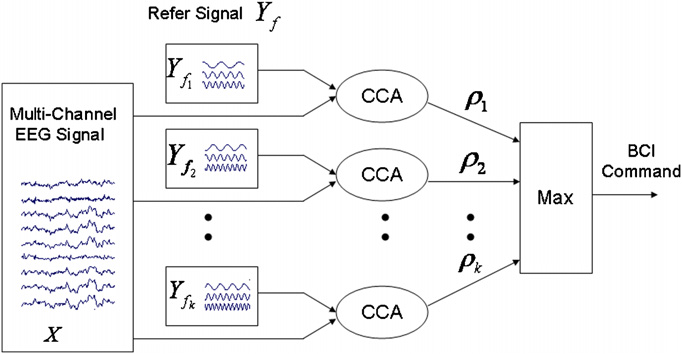
\includegraphics[width=0.7\textwidth]{cca.png}
	\caption{The visualisation of the steps of CCA feature extraction method~\cite{bin2009cca}.}
	\label{fig:cca}
\end{figure}

These two \gls{feature extraction} methods described in this chapter can be used as separate \gls{feature extraction} methods, but in the application described in chapter~\ref{sec:SSVEP_BCI}, these two methods collaborate with each other and therefore work as a single \gls{feature extraction} method.
